\chapter{Probabilistic rules}
\label{chap:rules}
\index{probabilistic rule|textbf}

The previous chapter fleshed out how dialogue could be represented as a stochastic process and argued for the use of probabilistic graphical models to efficiently encode the probability and utility models employed in dialogue management. Plain graphical models, however, must face non-trivial scalability issues when applied to dialogue domains associated with rich conversational contexts. The number of parameters necessary to perform dialogue state update and action selection can indeed increase rapidly with the complexity of the domain models. Alas, only small quantities of genuine training data are available in most dialogue domains, and usually cover only a small fraction of the state--action space of interest. 

To address this discrepancy between the size of the parameter space and the amount of data available to estimate them, we introduce in this chapter a new approach to probabilistic dialogue modelling, based on the notion of \textit{probabilistic rules}.  Probabilistic rules are structured mappings between conditions and effects, and function as \textit{high-level templates} for the construction of a dynamic decision network.  The key advantage of this structured modelling approach is the drastic reduction of the number of parameters compared to traditional representations.  We also argue that these expressive representations are particularly well suited to encode the probability and utility models of dialogue domains, where substantial amounts of expert knowledge can often be leveraged to structure the relationships between variables. 

The chapter is divided in six sections. Section \ref{sec:rmotivation} exposes in general terms how structural assumptions can be applied to reduce the size and complexity of probabilistic models.  Section \ref{sec:formalisation} defines our novel formalism of probabilistic rules and its main theoretical properties.  These definitions are then connected in Section \ref{sec:ruleinstantiation} to the graphical models described in the previous chapter by showing how the rules are instantiated in the Bayesian network representing the dialogue state. Section \ref{sec:processing-workflow} explains how this instantiation procedure is practically employed to update the current dialogue state and perform action selection. Finally, Section \ref{sec:amodelling} addresses some advanced modelling questions and Section \ref{sec:relatedwork} relates our approach to previous work.


\section{Structural leverage}
\label{sec:rmotivation}

The starting point of our approach is the observation that the probability and utility models used in dialogue management often exhibit a fair amount of \textit{internal structure}.  
We have already discussed in the previous chapter one simple instance of this internal structure, namely factored representations based on conditional independences. However, the internal structure of dialogue domains does not limit itself to these basic independence assumptions, and much can be gained by exploiting other types of structural properties, as shall be argued on the next pages. 

%If two sets of random variables $\mathbf{X}$ and $\mathbf{Y}$ are conditionally independent given $\mathbf{Z}$, we can rewrite the probability distribution $P(\mathbf{X}, \mathbf{Y} \, | \, \mathbf{Z})$ as $P(\mathbf{X} \, | \, \mathbf{Z}) (\mathbf{Y} \, | \, \mathbf{Z}) $.  


\subsubsection*{Latent variables}
 \index{latent variables}
The number of parameters required to estimate the distributions of a graphical model can often be reduced by introducing \textit{latent variables} (i.e.\ unobserved or hidden variables) that act as intermediaries between the source and target variables. Indeed, many application domains are often best explained by the combination of a small number of distinct factors or influences, each encoded by a separate random variable and associated with a subset of input and output variables. This layer of latent variables is usually never observed directly, but can contribute to structuring the model.\footnote{The construction of layered computational models is one of the most active research areas in artificial intelligence and machine learning and form the foundations of deep learning approaches \citep{Bengio:2009}.} In the domain of medical diagnosis, the relations between predisposing factors and observed symptoms are for instance best described by postulating an intermediary layer of variables -- possible diseases -- that mediates between the predisposing factors and the observed symptoms.  Figure \ref{fig:latentvariables} illustrates how latent variables can be exploited to provide an additional layer of abstraction within a graphical model.

 \begin{figure}[ht]
\centering
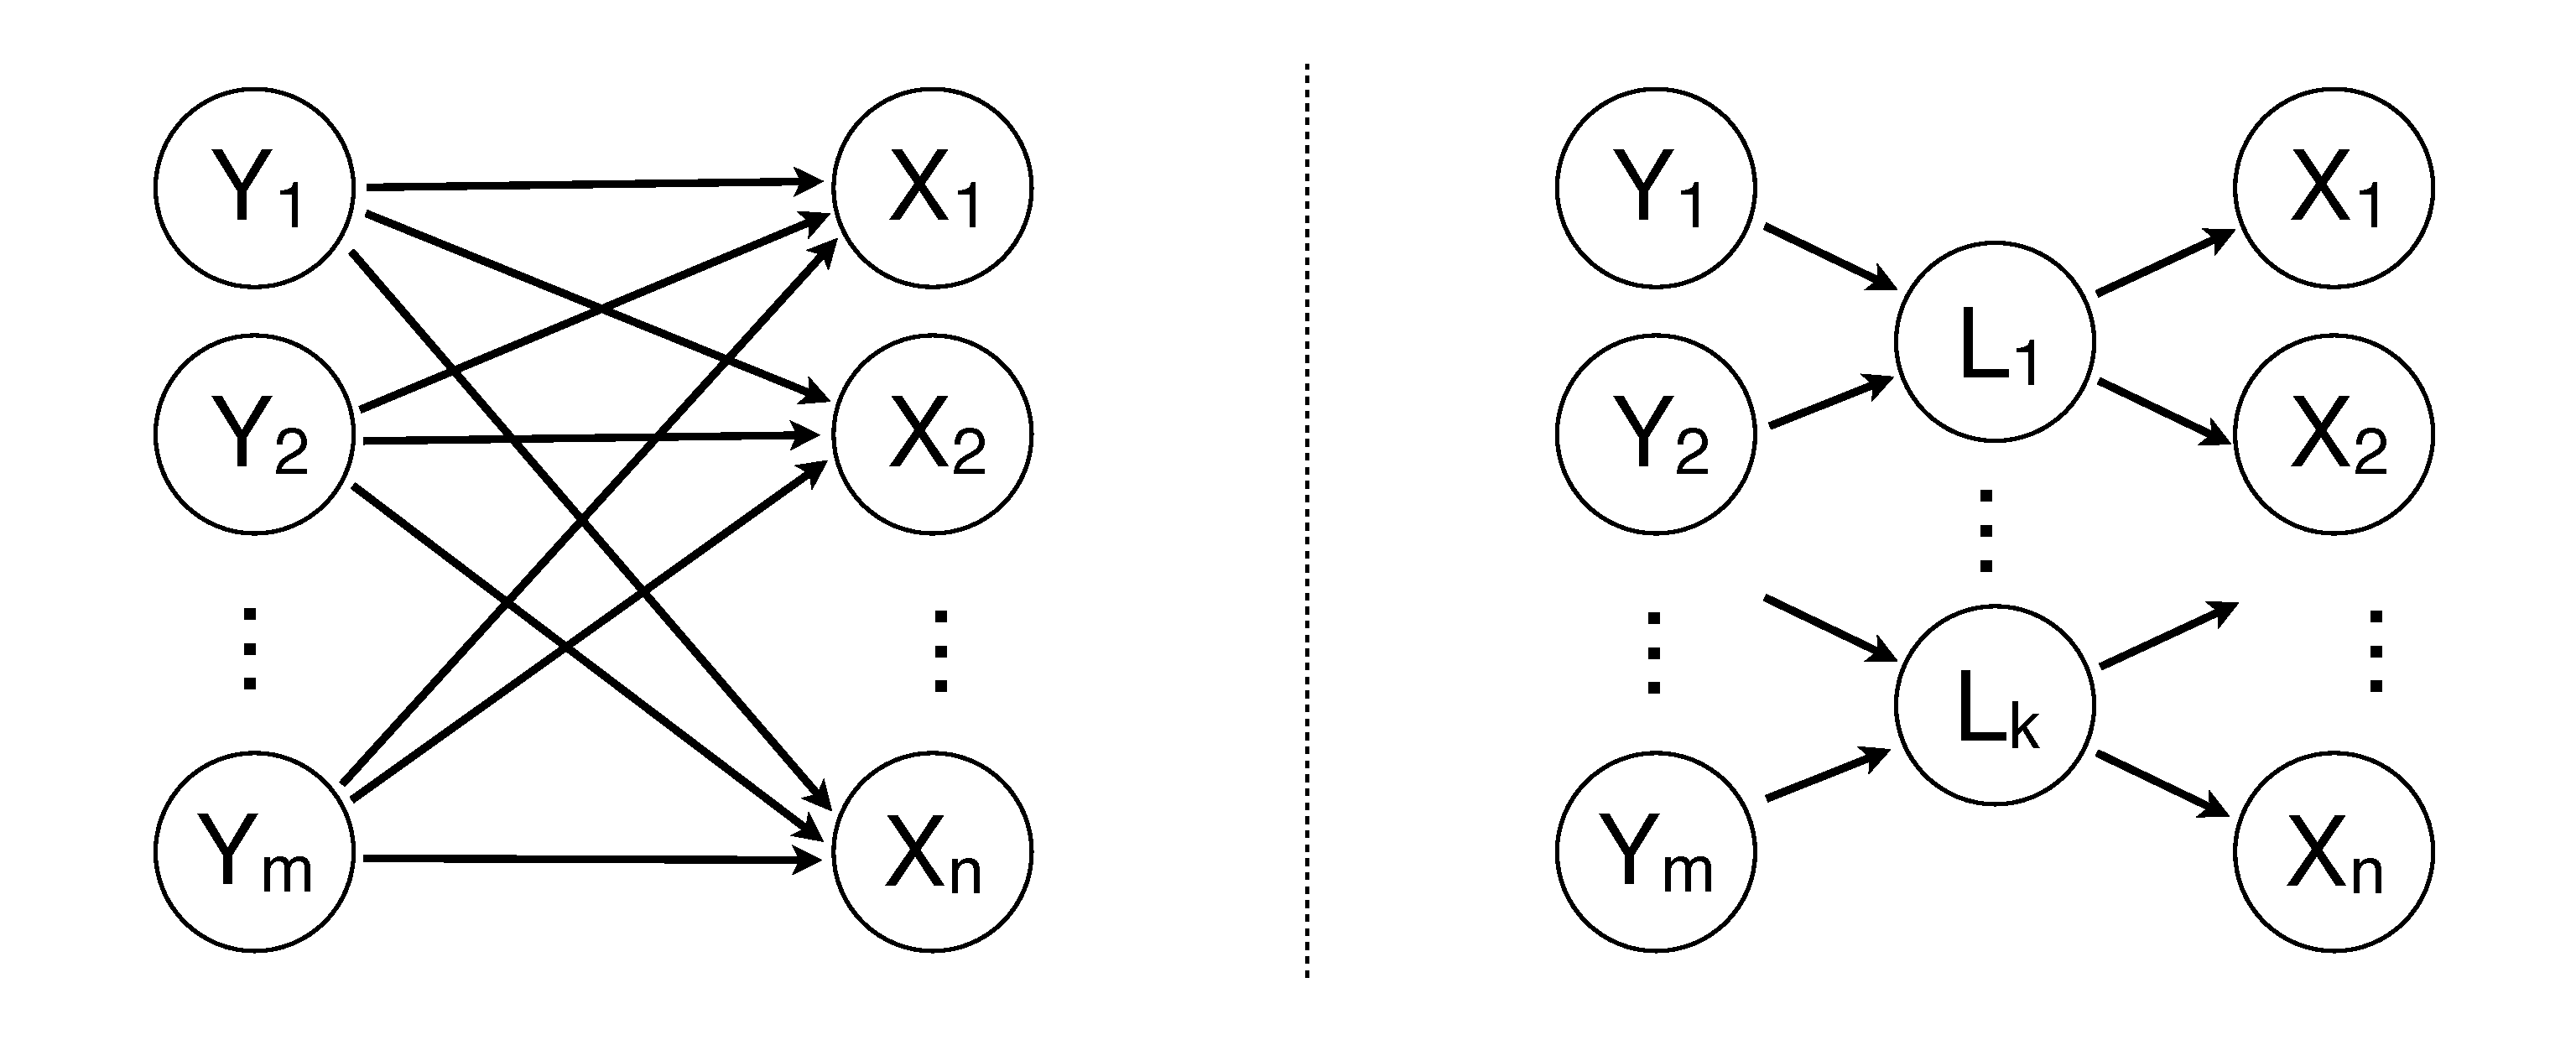
\includegraphics[scale=0.25]{imgs/latentvariables.pdf}
\caption{Comparison between a model that directly maps variables $\mathbf{Y}$ to $\mathbf{X}$ (left side) and one relying on latent variables $\mathbf{L}$ to serve as intermediaries (right side).}
\label{fig:latentvariables}
\end{figure}

Dialogue models can benefit from the inclusion of such latent variables. The transition function can for instance be modelled in terms of a limited number of latent variables, each responsible for capturing specific aspects of the interaction dynamics.  We shall see in the forthcoming sections that probabilistic rules precisely operate as latent variables when instantiated in the dialogue state. 

\subsubsection*{Partitioning}
\index{state space!partitioning of}
A random variable $X$ with parent variables $Y_1,\dots, Y_m$ must specify a separate probability distribution for every possible assignment of values for the parent variables. In other words, the number of parameters required to specify the distribution $P(X \, | \, Y_1, \dots, Y_m)$ is exponential in the number of parents $m$. Fortunately, the values of these parent variables can be grouped into \textit{partitions} yielding similar outcomes for $X$. One can therefore directly define the conditional probability distributions on these groups rather than on the full enumeration of combined values for the parent variables. Partitioning is an example of an \textit{abstraction mechanism} which can be used to reduce the model complexity and improve its ability to generalise to unseen examples. Partitioning is closely related to the notions of state abstraction and state aggregation in the reinforcement learning and planning literature \citep{conf/isaim/LiWL06}.  State abstraction/aggregation is the process of mapping a large state space into a more compact, abstract state space (corresponding here to the partitions).\index{state abstraction}

%Utility distributions can also partition the values of their dependent variables in a similar way.  

Figure \ref{fig:partitioning} illustrates such a partitioning operation for the conditional probability distribution $P(\mathit{Fire} \, | \mathit{Weather}, \mathit{Rain})$.  The space of possible values for the parent variables is defined in this example as $\mathit{Val}(\mathit{Weather}) \times \mathit{Val}(\mathit{Rain})$ and contains 6 possible elements.  We can observe that this space can be split in two partitions: $\mathit{Rain}\!=\mathit{true} \lor \mathit{Weather}\!\neq\mathit{hot}$ and $\mathit{Rain}\!=\mathit{false} \land \mathit{Weather}\!=\mathit{hot}$. This partitioning allows a significant reduction of the number of parameters required for the conditional probability distribution.  However, it should be noted that grouping value assignments into partitions corresponds to a modelling choice and can degrade the model accuracy if the partitions do not reflect actual similarities in the predicted outcomes.

%As illustration, consider a minimalistic dialogue in a robot learning scenario where the robot can ask the user yes/no questions pertaining to the colour of one specific object (e.g.\ \utt{Is the object red?}). In this simple scenario, the state is represented with two variables: the user dialogue act $a_u = \{\mathit{yes,no}\}$ and a variable representing the object colour, $\mathit{colour} = \{\mathit{blue,green, ...}\}$ with $n$ possible colours.  The system actions take the form $a_m = \{ \mathit{VerifyColour(c)}: c \in \mathit{colour}\}$, where $VerifyColour(c)$ corresponds to asking the user whether the object is of colour $c$.  Since the object colour remains constant, the transition function for this domain is defined as $P(a_u'|a_m, \mathit{colour})$. The number of parameters required to specify the transition function is $n^2$ (since $a_m$ and $\mathit{colour}$ have $n$ possible values each). 

%However, one can reasonably assume in this example that the particular colour mentioned in the question is irrelevant to predict the next user dialogue act $P(a_u'|a_m,\mathit{colour})$ as long as it matches (or fails to match) the actual colour of the object.  Based on this assumption, one can divide the space $\mathit{Val}(a_m) \times \mathit{Val}(\mathit{colour})$ into two distinct partitions: 
%\begin{enumerate}
%\item One partition in which the verification question corresponds to the actual colour of the object: $\exists c: colour\!=\!c \land a_m\!=\!\mathit{VerifyColour(c)}$.
%\item One partition in which there is a mismatch between the colour mentioned in the question and the actual colour: $\exists c: colour\!=\!c \land a_m\!\neq\!\mathit{VerifyColour(c)}$.
%\end{enumerate}

%By abstracting over the specific colour mentioned in the question, partitioning allows us to drastically reduce the number of parameters required for the conditional probability distribution $P(a_u'|a_m,\mathit{colour})$ from a total of $n^2$ to only $2$. Figure \ref{fig:partitioning} illustrates this reduction. 


 \begin{figure}[ht]
\centering
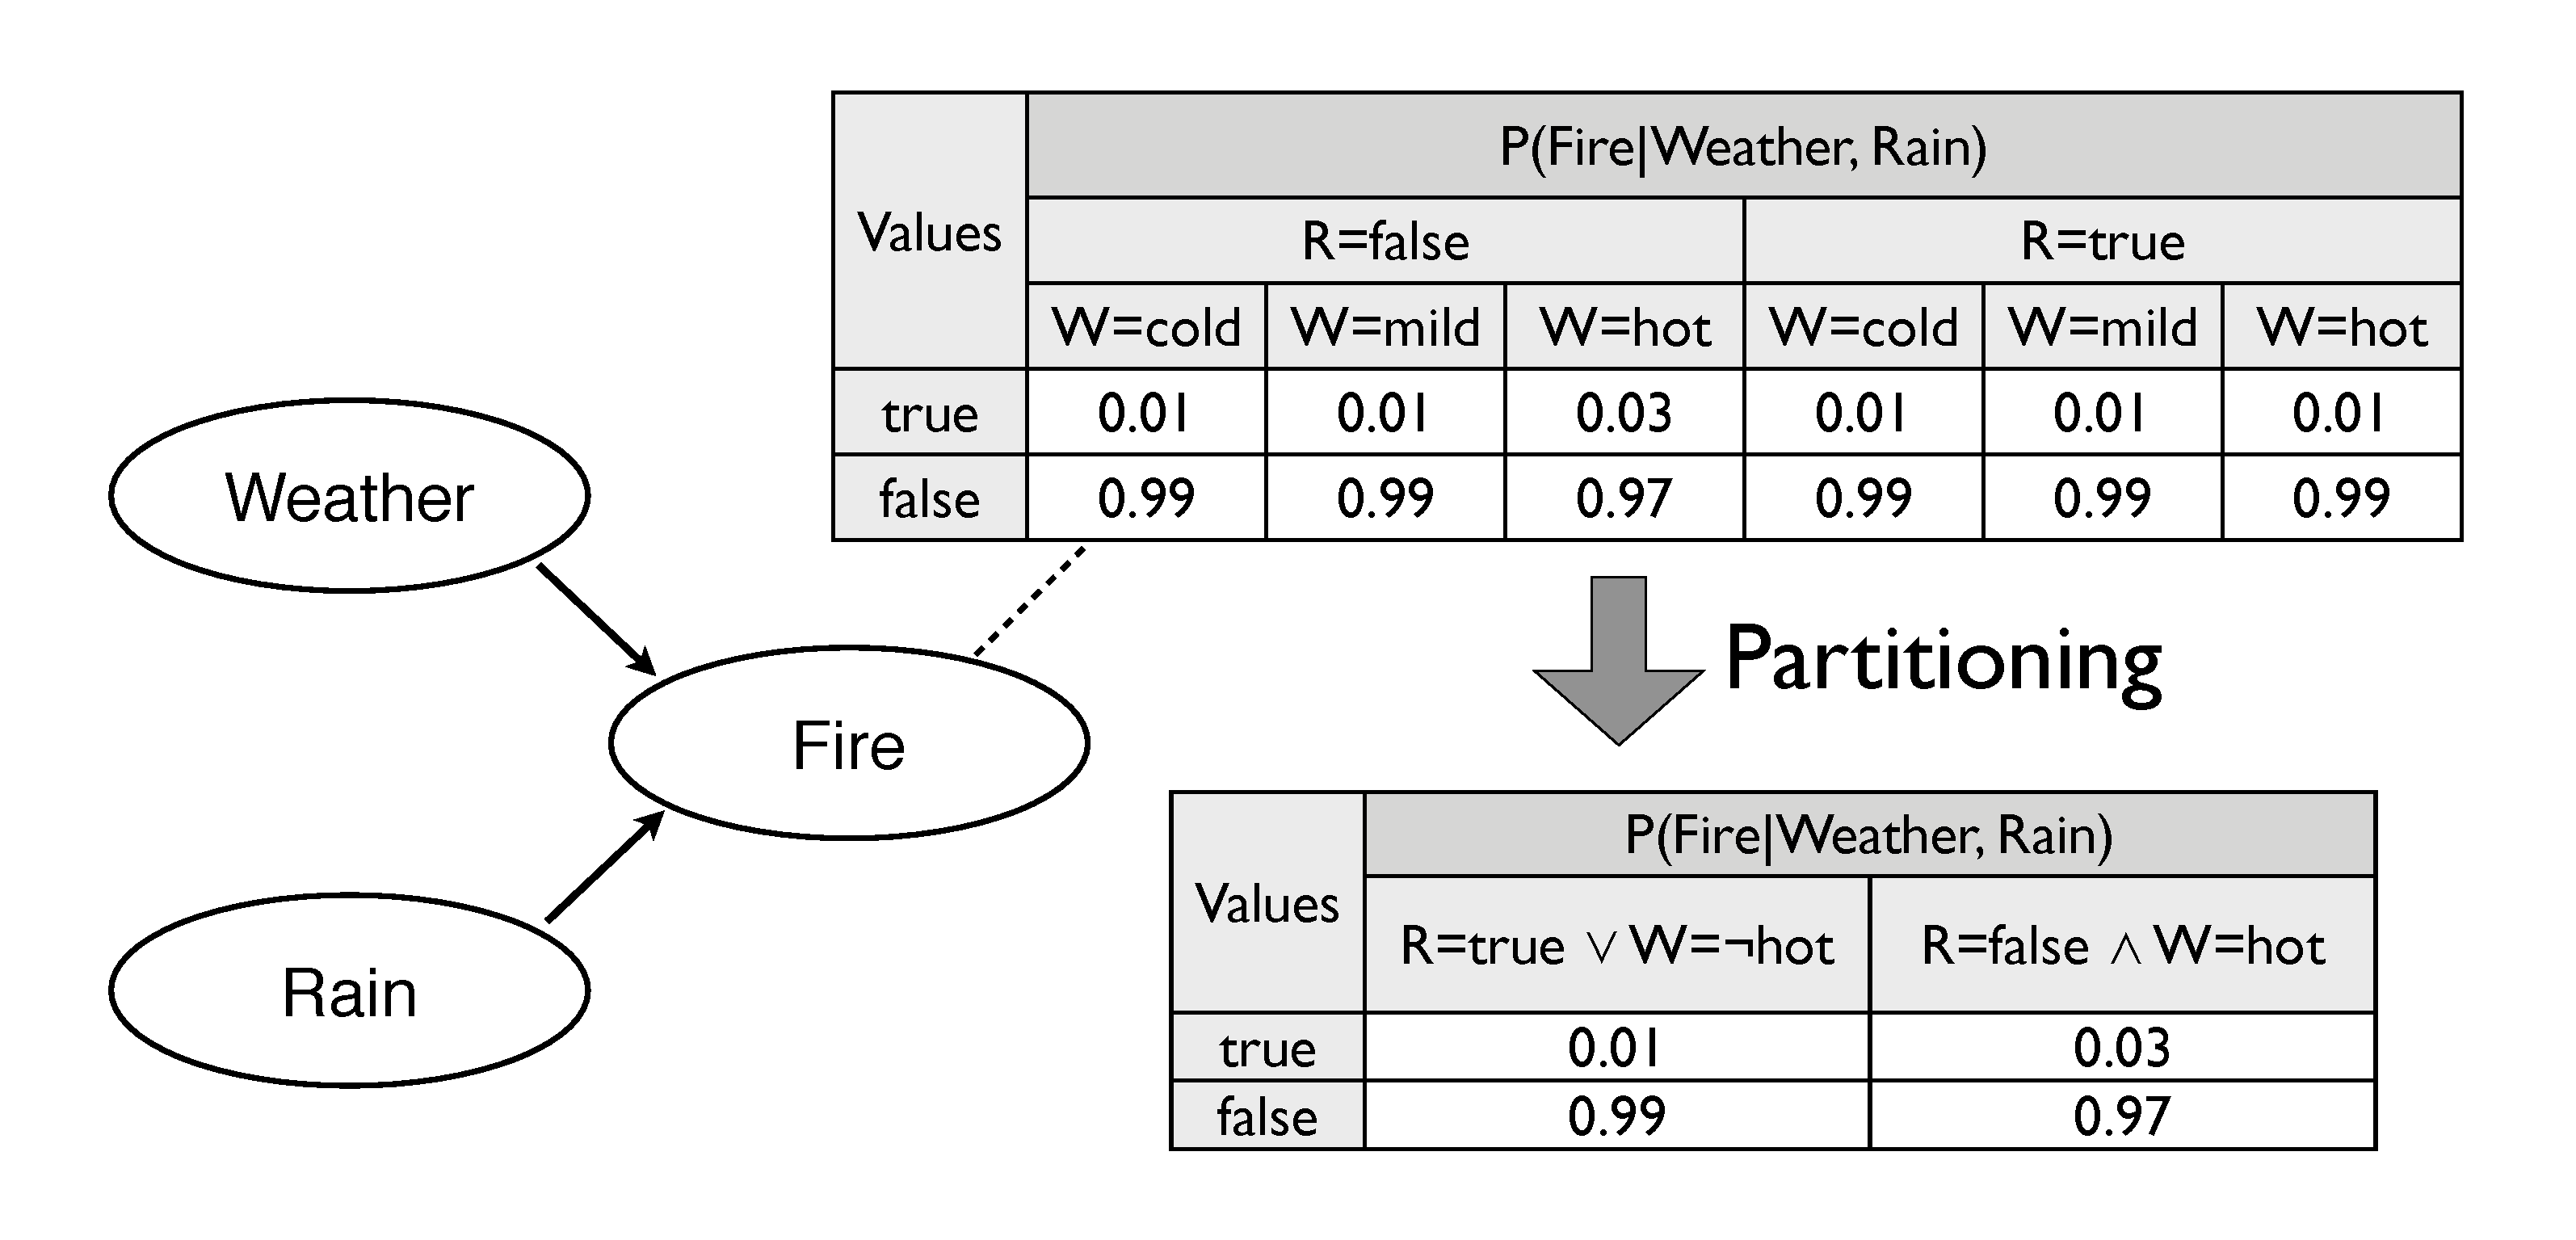
\includegraphics[scale=0.25]{imgs/partitioning.pdf}
\caption{Partitioning for the conditional probability distribution $P(\mathit{Fire} \, | \mathit{Weather}, \mathit{Rain})$.}
\label{fig:partitioning}
\end{figure}

Partitions must be both exhaustive (each combination of values for the parent variables must belong to one partition) and mutually exclusive (a combination of values can only belong to one partition).  As we can observe from the example, partitions can often be concisely expressed via logical conditions on the variable values.  A given assignment of values is then grouped in a partition if it satisfies the condition associated with it. 

\subsubsection*{Quantification}
\index{quantification}

Many dialogue domains are composed of objects or entities related to one another. These domains are often difficult to directly represent with a fixed set of random variables, as the number of entities and relations may vary over time.  Examples of relational structures include: 
\begin{itemize}
\item Collections of physical objects in a visual scene, each described by specific features (colour, shape) and relations with other objects (e.g.\ spatial relations).
\item Indoor environments topologically structured in rooms and spaces in which to navigate. 
\item Collections of tasks to complete by the agent, each task being possibly connected to other tasks via precedence or inclusion relationships.
\item Linguistic entities employed in the dialogue acts of a given interaction, linked with one another through multiple syntactic, semantic, referential or pragmatic relations. 
\end{itemize}

\textit{First-order logic}\index{first-order logic} provides an excellent basis for representing and manipulating such relational structures, as it offers a mathematically principled language for (1) referring to objects connected with one another through functions and relations and (2) describing their properties in a concise way through the use of universal and existential quantifiers.\footnote{We shall not cover in this thesis the mathematical foundations of first-order logic, but the reader is invited to refer to e.g.\ \cite{gamut1991logic} for a formal overview of the logical concepts mentioned throughout this thesis.}

Graphical models represent relational domains by instantiating one random variable for every possible grounding of the functions and predicates defined for the domain for a collection of objects.\footnote{Such an operation is akin to \textit{propositionalisation} in the terminology of first-order logic.}  A domain with two objects $o_1$ and $o_2$ and a relation $\mathit{leftOf}(x,y)$ will for instance generate the four groundings $\mathit{leftOf}(o_1,o_2)$, $\mathit{leftOf}(o_2,o_1)$, $\mathit{leftOf}(o_1,o_1)$ and $\mathit{leftOf}(o_2,o_2)$. The definition of probability and utility distributions that can capture the relational semantics of such a representation can, however, be problematic. In particular, universal properties and constraints such as $\forall x, \neg \mathit{leftOf}(x,x)$ and $\forall x, y, z, \mathit{leftOf}(x,y) \land \mathit{leftOf}(y,z) \Rightarrow \mathit{leftOf}(x,z)$ can be difficult to enforce at a global level, since classical probabilistic models are intrinsically limited to propositional logic and offer no direct support for quantifiers. 
 
The unification of first-order logic and probability theory has spanned a new research area called \textit{statistical relational learning}\index{statistical relational learning} \citep{getoor:srlbook07}. A common trait of most approaches to statistical relational learning is the definition of a logic-based description language which is employed as a template to generate classical probabilistic models given a set of constants. The introduction of quantifiers provides an abstraction mechanism to reduce the complexity of probability and utility models by describing constraints or relations that hold for all possible groundings of a given formula and can therefore apply to large sets of random variables. 

\section{Formalisation}
\label{sec:formalisation}

We now introduce a new, generic modelling framework for expressing the various types of internal structure we have just detailed.  This framework revolves around the notion of \textit{probabilistic rules}. The framework was originally presented in \cite{rulebasedmodels-sigdial2012,lison-semdial2012}. The following sections present the framework and its application to dialogue management.  The framework will then be discussed and compared to related approaches in Section \ref{sec:relatedwork}.

The key idea is to represent distributions with the help of \textit{if...then...else} constructions, based on the following skeleton:\index{probabilistic rule}
\begin{equation*}
\begin{aligned}
& \textbf{if} \ \ (\text{condition 1 holds}) \ \ \textbf{then} \\ 
& \;\;\;\;\; \text{Distribution 1 over possible effects} \\
& \textbf{else if} \ \ (\text{condition 2 holds}) \ \ \textbf{then} \\ 
& \;\;\;\;\; \text{Distribution 2 over possible effects} \\
& ... \\
& \textbf{else} \\
& \;\;\;\;\; \text{Distribution } n \text{ over possible effects} \\ 
\end{aligned}
\end{equation*}

Each \textit{if...then} branch specifies both a \textit{condition} on particular state variables and an associated distribution over possible \textit{effects}.   The \textit{if...then...else} construction is read in sequential order, as in programming languages, until a satisfied condition is found, which causes the activation of the corresponding probabilistic effects. 

We first present how probabilistic rules can express conditional probability distributions in terms of structured mappings between input and output variables.  We then show how to  generalise the formalism to utility distributions and extend it with quantification mechanisms.

A terminological note is at this point in order: We shall use the term \textit{probabilistic rules} as an umbrella term that covers all types of rules in this thesis, while \textit{probability rules} will only refer to rules expressing probability distributions over effects, and \textit{utility rules} to rules expressing utility distributions.

\subsection{Probability rules}
\label{sec:probabirules}
\index{probability rule}

Probability rules take the form of \textit{if...then...else} constructions and map a list of conditions on input variables to probabilistic effects on output variables. More formally, a rule is expressed as an ordered list $[ br_1, \dots, br_{n}]$ in which $br_i$ denotes the $i$-th branch of the \textit{if...then...else}. Each branch $br_i$ is a pair $\langle c_i, P(E_i) \rangle$ where $c_i$ is a logical condition and $P(E_i)$ an associated categorical distribution over a range of possible effects $\mathit{Val}(E_i) = \{e_{(i,1)}, \dots, e_{(i,m_i)}\}$.  The value $m_i$ corresponds to the number of alternative effects in $P(E_i)$.  Each effect $e_{(i,j)} \in \mathit{Val}(E_i)$ has a particular probability denoted $p_{(i,j)}$. 

Given these elements, a probability rule reads as such:\index{probability rule!structure of}
\begin{equation}
\begin{aligned}
& \textbf{if} \ \ (c_{1}) \ \ \textbf{then} \\ 
& \;\;\;\;\; \begin{cases}
P(E_1\!=\!e_{(1,1)}) = p_{(1,1)} \\
 \dots \\
P(E_1\!=\!e_{(1,m_1)}) = p_{(1,m_1)} 
\end{cases} \\[3mm]
& \textbf{else if} \ \ (c_{2}) \ \ \textbf{then} \\ 
& \;\;\;\;\; \begin{cases}
P(E_2\!=\!e_{(2,1)}) = p_{(2,1)} \\
 \dots \\
P(E_2\!=\!e_{(2,m_2)}) = p_{(2,m_2)}
\end{cases} \\ 
& \dots  \\
& \textbf{else} \\
& \;\;\;\;\; \begin{cases}
P(E_{n}\!=\!e_{(n,1)}) = p_{(n,1)} \\
\dots \\
P(E_{n}\!=\!e_{(n,m_n)}) = p_{(n,m_n)}
\end{cases}
\end{aligned}
\label{eq:probrule}
\end{equation}

We will often use $P(e_{(i,j)})$ as a notational convenience for $P(E_i = e_{(i,j)})$.   We describe below how the conditions $c_i$, effects $e_{(i,j)}$ and effect probabilities $p_{(i,j)}$ are respectively defined. 

\subsubsection*{Conditions}
\index{probabilistic rule!conditions of}

The conditions $c_i$ are expressed as logical formulae grounded in a subset of random variables in the dialogue state. Conditions can be arbitrarily complex logical formulae connected by conjunction, disjunction and negation.  The list of random variables mentioned in the condition corresponds to the \textit{input variables} of the rule, which we shall denote as $I_1, \dots, I_{k}$. Table \ref{table:syntaxconditions} details the syntax of a rule condition.  The input variables and values are arbitrary terms for the domain and (as shall be explained in Section \ref{sec:quantification}) can also include free variables in addition to ground terms. 

The two examples $(\mathit{Rain}\!=\mathit{true} \lor \mathit{Weather}\!\neq\mathit{hot})$ and $(\mathit{Rain}\!=\mathit{false} \land \mathit{Weather}\!=\mathit{hot})$ in Figure \ref{fig:partitioning} are instances of valid conditions on the two input variables $Rain$ and $\mathit{Weather}$. 

Given that a rule is defined through an \textit{if...then...else} construction, the partitioning is guaranteed by construction to be exhaustive and mutually exclusive (only one branch will be followed).  When provided with an assignment of values on the input variables, the conditions are tested in sequential order until one is satisfied. When no terminating \textbf{else} block is explicitly specified at the end of a rule, the framework assumes a final \textbf{else} block associated with a void effect to ensure that the partitioning is exhaustive. The last condition $c_n$ is thus guaranteed to always be trivially satisfied irrespective of the input variable values. The partitioning automatically follows from the rule structure as an \textit{if...then...else} construction, and the conditions $c_1,\dots, c_n$ themselves need not be mutually exclusive. 

The conditions on the input variables offer a compact partitioning of the state space to mitigate the dimensionality curse.  Without this partitioning in alternative conditions, a rule ranging over the input variables $I_1, \dots, I_{k}$ would need to enumerate $\mathit{Val}(I_1) \times \dots \times \mathit{Val}(I_k)$ possible assignments.  Partitioning this space reduces this number to $n$ partitions, where $n$ corresponds to the number of conditions for the rule and is usually small. 


\setlength{\grammarindent}{12em} 

\begin{table}[h]
\vspace{3mm}
\begin{grammar}

<Condition> ::= <AtomicCondition> | <ComplexCondition> | \ `true'

<AtomicCondition> ::= <InputVariable> <BinaryOperator> <Value>

<ComplexCondition> ::= \lit{(} <Condition> \lit{)} 
\alt \lit{$\lnot$} <Condition> 
\alt <Condition> \lit{$\land$} <Condition> 
\alt <Condition> \lit{$\lor$} <Condition>

<BinaryOperator> ::= `=' | \lit{$\neq$} | `\textless' | `\textgreater'

<InputVariable> ::= term of the domain

<Value> ::= term  of the domain

\end{grammar}
\caption{Syntax (in Bachus--Naur form) of a rule condition.}
\label{table:syntaxconditions}
\end{table}

\subsubsection*{Effects}
\index{probabilistic rule!effects of}

Associated to each condition $c_i$ stands a collection of possible effects $e_{(i,1)}, \dots, e_{(i,m_i)}$. Each effect $e_{(i,j)}$ represents a specific assignment of values for a set of variables called the \textit{output variables} of the rule.  An effect is formally defined as an assignment of values $O_1'\!=\!o_1 \land \dots \land O_{l}'\!=\!o_{l}$ where $O_1', \dots, O_{l}'$ denote the output variables and $o_1, \dots, o_{l}$ the corresponding values assigned to these variables. Effects can be void -- that is, represent an empty assignment. We shall adopt throughout this thesis the convention of denoting output variables with a prime to distinguish them from other types of variables. 

Table \ref{table:syntaxeffects} details the syntax of a rule effect. In the example from Figure \ref{fig:partitioning}, the output variable is a singleton and corresponds to $Fire$. We shall, however, encounter examples of rules with more than one output variable. As for the rule conditions, the output variables and values correspond to arbitrary terms of the domain, and can also include free variables. 


\begin{table}[h]
\vspace{3mm}
\begin{grammar}

<Effect> ::= <NonVoidEffect> | \ $\emptyset$

<NonVoidEffect> ::= <AtomicEffect> | <NonVoidEffect> \lit{$\land$} <NonVoidEffect> 

<AtomicEffect> ::= <OutputVariable> `=' <Value>

<OutputVariable> ::= term of the domain

<Value> ::= term  of the domain

\end{grammar}
\caption{Syntax (in Bachus--Naur form) of a rule effect.}
\label{table:syntaxeffects}
\end{table}

\subsubsection*{Probabilities}

Each effect $e_{(i,j)}$ in the categorical probability distribution $P(E_i)$ is assigned with a probability $p_{(i,j)} = P(E_i = e_{(i,j)})$ that must satisfy the usual probability axioms.  The probabilities can be either fixed by hand or estimated empirically (as will be demonstrated in Chapters \ref{chap:wozlearning} and \ref{chap:rllearning}).

%In the latter case, we adopt a Bayesian learning approach (cf. Section \ref{sec:learning}) and assume the probabilities $p_i^{1...m_i}$ to be drawn from the conjugate prior of categorical distributions, namely Dirichlet distributions.

\subsubsection*{Example}

Rule $r_1$ illustrates a simple example of a probability rule:
\begin{align*}
r_1: \ \ \ \ \ & \textbf{if} \ (\mathit{Rain}\!=\!\mathit{false} \land \mathit{Weather}\!=\!\mathit{hot}) \ \textbf{then} \\
& \;\;\;\;\;  \begin{cases}
 P(\mathit{Fire}'\!=\!\mathit{true}) = 0.03 \\ 
P(\mathit{Fire}'\!=\!\mathit{false}) = 0.97
\end{cases} \\ 
& \textbf{else} \\
& \;\;\;\;\; \begin{cases}
P(\mathit{Fire}'\!=\!\mathit{true}) = 0.01 \\
P(\mathit{Fire}'\!=\!\mathit{false}) = 0.99
\end{cases} 
\end{align*}

Rule $r_1$ has two input variables: $\mathit{Rain}$ and $\mathit{Weather}$ as well as one output variable $\mathit{Fire}'$. The rule specifies that the probability of a fire is 0.03 in case of no rain and a hot weather and 0.01 in all other cases.  The rule structure enables the conditional probability distribution for $\mathit{Fire}'$ to be specified with only 4 probabilities in comparison to 12 for the probability distribution shown in Figure \ref{fig:partitioning}. 

%Here is a first example of probabilistic rule pertaining to the user action model: 
%\begin{align*}
%\textbf{Rule 1}: \ \ & \textbf{if} \ (\exists X: a_m=\mathit{Confirm(X)} \land i_u = \mathit{X})  \ \textbf{then} \\ 
%& \;\;\;\;\; \{[P(a_u' = \mathit{Confirm}) = 0.9]\} \\
%& \textbf{else if} \ (\exists X: a_m=\mathit{Confirm(X)} \land i_u \neq \mathit{X})  \ \textbf{then} \\ 
%& \;\;\;\;\; \{[P(a_u' = \mathit{Disconfirm}) = 0.95]\}
%\end{align*}
%The rule specifies that, if the system requests the user to confirm that his intention is $X$ and his actual intention is indeed $X$, the user is expected to utter a $\mathit{Confirm}$ action with probability 0.9.  Otherwise, the rule produces a void effect -- i.e.\ it leaves the distribution $P(a_u')$ unchanged. If the intention is different, the user will utter a $\mathit{Disconfirm}$ action with  probability 0.95.   

\subsection{Utility rules}
\index{utility rule}

The rule-based formalism we have outlined can also be used to express utility distributions with only minor notational changes. Utility rules essentially retain the same form as probability rules, with one important exception, namely that the probabilistic effects are replaced by utility distributions over particular assignments of decision variables. 

Formally, a utility rule is an ordered list $[ br_1, \dots, br_n]$, where each branch $br_i$ is a pair $\langle c_i, U_i \rangle$, $c_i$ is a condition and $U_i$ an associated utility table over possible assignments of decision variables. The utility distribution $U_i$ specifies a set of possible decisions $d_{(i,1)}, \dots, d_{(i,m_i)}$.  Each decision $d_{(i,j)}$ has a particular utility value denoted $u_{(i,j)}$.  Utility rules can be expressed in the following manner:\index{utility rule!structure of}
\begin{equation}
\begin{aligned}
& \textbf{if} \ \ (c_{1}) \ \ \textbf{then} \\ 
& \;\;\;\;\; \begin{cases}
U_1(d_{(1,1)}) = u_{(1,1)} \\
 \dots \\
U_1(d_{(1,m_1)}) = u_{(1,m_1)} 
\end{cases} \\[3mm]
& \textbf{else if} \ \ (c_{2}) \ \ \textbf{then} \\ 
& \;\;\;\;\; \begin{cases}
U_2(d_{(2,1)}) = u_{(2,1)} \\
 \dots \\
U_2(d_{(2,m_2)}) = u_{(2,m_2)} 
\end{cases} \\
& \dots  \\
& \textbf{else} \\
& \;\;\;\;\; \begin{cases}
U_n(d_{(n,1)}) = u_{(n,1)} \\
 \dots \\
U_n(d_{(n,m_n)}) = u_{(n,m_n)}
\end{cases}
\end{aligned}
\end{equation}

A utility rule assigns utility values to particular system decisions depending on conditions on the state variables.  As for probability rules, the conditions $c_i$ are defined as arbitrary logical formulae on input variables $I_1, \dots, I_k$.  The decisions $d_{(i,j)}$ are assignments $D_1'\!=\!D_1 \land \dots \land A_{l}'\!=\!a_{l}$ where the variables $D_1',..A_{l}'$ are decision variables and $d_1, \dots, a_{l}$ possible values for these variables. Similarly to the output variables of probability rules, we shall always denote decision variables with a prime. The utility values $u_{(i,j)}$ are real numbers (which may be positive or negative).  

Although most utility rules only include one single decision variable, the possibility to integrate multiple decision variables is helpful in domains where the system can execute multiple actions in parallel. Such situations can arise in human--robot interaction and multi-modal applications, as the system can communicate through both verbal and non-verbal channels and is often able to perform physical actions in addition to communicative acts. 
 
\subsubsection*{Example}

Rule $r_2$ provides a simple example of a utility rule:
\begin{align*}
r_2: \ \ & \textbf{if} \ (\mathit{Fire}\!=\!\mathit{true}) \ \textbf{then} \\
& \;\;\;\;\;  \begin{cases}
U(\mathit{Tanker}'\!=\!\mathit{drop\mbox{-}water}) = 5 \\
U(\mathit{Tanker}'\!=\!\mathit{wait}) = -5
\end{cases} \\
& \textbf{else} \\
& \;\;\;\;\; \begin{cases}
U (\mathit{Tanker}'\!=\!\mathit{drop\mbox{-}water}) = -1 \\
U(\mathit{Tanker}'\!=\!\mathit{wait}) = 0
\end{cases}
\end{align*}

Rule $r_2$ stipulates the respective utilities of the two possible utility values for the decision variable $\mathit{Tanker}'$ depending on the input variable $\mathit{Fire}$. 

\subsection{Quantification}
\label{sec:quantification}
\index{probabilistic rule!quantifiers in}
\index{first-order logic}

Quantification is a powerful mechanism to abstract over particular relational aspects of the domain structure.  Free variables can be included in the specification of both the conditions and effects of a given rule and are universally quantified on top of the rule.\footnote{These free variables are variables in the sense of first-order logic, and are not to be confused with the random variables of the probabilistic model.}  A rule containing the free variables $y_1 \dots, y_p$ in its conditions and/or effects is therefore formalised as:
\begin{equation}
\begin{aligned}
\forall \ y_1, y_2, \dots, y_p, \\
& \textbf{if} \ \ (c_{1}) \ \ \textbf{then} \\ 
& \;\;\;\;\; \begin{cases}
P(E_1\!=\!e_{(1,1)}) = p_{(1,1)} \\
 \dots \\
P(E_1\!=\!e_{(1,m_1)}) = p_{(1,m_1)} 
\end{cases} \\[3mm]
& \textbf{else if} \ \ (c_{2}) \ \ \textbf{then} \\ 
& \;\;\;\;\; \begin{cases}
P(E_2\!=\!e_{(2,1)}) = p_{(2,1)} \\
 \dots \\
P(E_2\!=\!e_{(2,m_2)}) = p_{(2,m_2)} 
\end{cases} \\ 
&  \dots  \\
& \textbf{else} \\
& \;\;\;\;\; \begin{cases}
P(E_n\!=\!e_{(n,1)}) = p_{(n,1)} \\
 \dots \\
P(E_n\!=\!e_{(n,m_n)}) = p_{(n,m_n)}
\end{cases}
\end{aligned}
\label{eq:rulewithquant}
\end{equation}

The formalisation allows specific elements $y_1, \dots, y_p$ inside the conditions and effects of a rule to be \textit{underspecified}.\index{probabilistic rule!quantified variables in}  The mapping between conditions and effects specified by the rule is therefore duplicated for every possible assignment of the free variables.  Section \ref{sec:applicationquantif} explains how this finite set of possible assignments (also called the \textit{groundings} of the free variables) is practically determined on the basis of the current state. 

Based on this quantification mechanism, probabilistic rules can cover large portions of the state space in a highly compact manner, based on a reduced number of parameters. One of the main advantages of this representation is that it allows for powerful forms of \textit{parameter sharing}\index{parameter sharing}, since the effect probabilities $p_{(i,j)}$ in the above rule are made independent of the various instantiations of the variables $y_1, \dots, y_p$.  The quantification mechanism adopted in this thesis is similar to the one used in Markov logic networks \citep{Richardson:2006}, with the constraint that universal quantifiers are in this framework only allowed at the top of the rule.  In line with most approaches to statistical relational learning \citep{getoor:srlbook07} and logic programming \citep{Poole:2008}, the formalisation relies on a ``database semantics'' that assumes domain closure (the domain does not contain more elements than those explicitly specified). \index{database semantics}

Quantification also applies to utility rules in the same manner, through the inclusion of logical variables in the conditions $c_i$ and decisions $d_{(i,j)}$  of the utility rule. 

\subsubsection*{Example}

Rule $r_3$ provides a simple example of a probability rule including a quantified variable:
\begin{align*}
r_3: \ \ & \forall y, \\ 
& \textbf{if} \ (\mathit{shape}(y) = \mathit{sphere})  \ \textbf{then} \\ 
& \;\;\;\;\; \begin{cases}
P(\mathit{graspable}(y)'\!=\!\mathit{true}) = 0.9 \\
P(\mathit{graspable}(y)'\!=\!\mathit{false}) = 0.1
\end{cases} \\ 
&\textbf{else if} \ (\mathit{shape}(y) = \mathit{cone})  \ \textbf{then} \\ 
& \;\;\;\;\; \begin{cases}
P(\mathit{graspable}(y)'\!=\!\mathit{true}) = 0.2 \\
P(\mathit{graspable}(y)'\!=\!\mathit{false}) = 0.8
\end{cases}
\intertext{Rule $r_3$ specifies how the graspability of a given object $y$ depends on its shape (a sphere being easier to grasp than a cone). Similarly, rule $r_4$ defines the utility of a grasping action depending on the task and object graspability:}
r_4: \ \ & \forall y, \\ 
& \textbf{if} \ (task= grasp(y) \land \mathit{graspable}(y) = \mathit{true})  \ \textbf{then} \\ 
& \;\;\;\;\; \begin{cases}
U(a_m'\!=\!\mathit{grasp}(y)) = 2 \\
\end{cases} \\
&\textbf{else} \\
& \;\;\;\;\; \begin{cases}
U(a_m'\!=\!\mathit{grasp}(y)) = -2 \\
\end{cases} 
\end{align*}
Rule $r_4$ associates a utility of 2 to the action of grasping an object $y$ when the object is graspable and corresponds to the task to perform, and a utility of -2 in any other case.

%Grasping the object in any other case results in a negative utility of -2.  %The careful reader may notice that quantified variables are allowed  both inside the label of particular variables, as in $\mathit{graspable}(y)'$, as well as inside the variable values, as in $grasp(y)$.  

%Assume you want to predict the next user dialogue act $a_u'$ after a system-initiated question such as ``What colour is the object'' depending on the colour of the object that is referred to. Rule $r_3$ is an example of rule that employs quantification on two variables denoted $o$ and $c$.\footnote{Note the absence of an explicit final \textit{else} branch, which is then by default associated with an empty effect.}
%\begin{align*}
%r_3: \ \ & \forall o, c: \\ 
%& \textbf{if} \ (a_m\!=\!\mathit{WhatIsColour}(o) \land \mathit{colour}(o)\!=\!\mathit{c})  \ \textbf{then} \\ 
%& \;\;\;\;\; \begin{cases} P(a_u'=\mathit{AssertProperty}(o,\mathit{c})) = 0.95 \end{cases}
%\end{align*}

%Rule $r$ assumes the presence in the dialogue state of a random variable $colour(o_i)$ for each object $o_i$ perceived by the system.  The rule specifies that the user is likely (with probability 0.95) to utter a dialogue act such as ``the object is X'' at the next turn, where X is the actual colour of the object. Otherwise no prediction is made. If the dialogue state contains e.g.\ one object $o_1$ with $P(\mathit{colour}(o_1)=blue)=0.8$ and the last system action was $WhatIsColour(o_1)$, the probability of the user uttering ``the object is blue'' is therefore $0.76$.  

\section{Rule instantiation}
\label{sec:ruleinstantiation}
\index{probabilistic rule!instantiation of}

We represent the dialogue state\index{dialogue state} as a Bayesian network\index{Bayesian network} over state variables, in line with other dialogue management approaches such as \cite{Thomson:2010:BUD:1772996.1773040} and \cite{bui2009}. Rules are then applied at runtime on this dialogue state.  The instantiation is performed by creating a distinct node for every rule to apply. These rule nodes are essentially latent variables\index{latent variables} that serve as intermediaries between input and output variables.  Although the presence of these rules is never directly observed, they contribute to structuring the relations between variables and enable the system designer to decompose complex probability and utility models into smaller parts.   % The instantiated rules are equivalent to a dynamic decision network (cf. previous chapter). 

We describe below the instantiation procedure for each type of rule. For the sake of clarity, we shall first limit our discussion to rules without universal quantification, and then demonstrate how quantification can be accounted for in the instantiation process. 

\subsection{Probability rules}
\label{sec:probruleinstantiation}
\index{probability rule!instantiation of}

Let $\mathcal{B}$ be the Bayesian network representing the current dialogue state, and $\mathcal{R}$ a set of rules to apply to this dialogue state.  For each rule $r \in \mathcal{R}$, a distinct chance node is created.\footnote{The original instantiation algorithm presented in \citep{rulebasedmodels-sigdial2012} included two separate nodes: one for the rule condition and one for the effect.  The formalism was later simplified to one single node as we realised that only one node was necessary to represent the semantics of the rule.} This chance node represents a random variable defined on the possible effects of the rule.  The node is conditionally dependent on the input variables of the rule (i.e.\ the set of all variables that are mentioned in the rule conditions), and is also connected via outgoing edges to its output variables (i.e.\ the set of all variables that are mentioned in the rule effects). 

Figure \ref{fig:instantiationprob} illustrates this instantiation process on an abstract, constructed example composed of the two rules $r_5$ and $r_6$.  To simplify the rule representation, we shall usually omit the explicit specification of the probability for the empty effect in the effect distributions.  The remaining probability mass in each effect specification  is thus by default assigned to the empty effect.  The first $\mathbf{if}$ branch of rule $r_5$ has for instance an empty effect with probability 0.4.

The two rules $r_5$ and $r_6$ are applied on the state variables $A$, $B$, $C$ and $D$.  The application of the two rules results in an updated variable $A'$ and the creation of a new variable $E'$. 

\begin{figure}[ht]
\centering
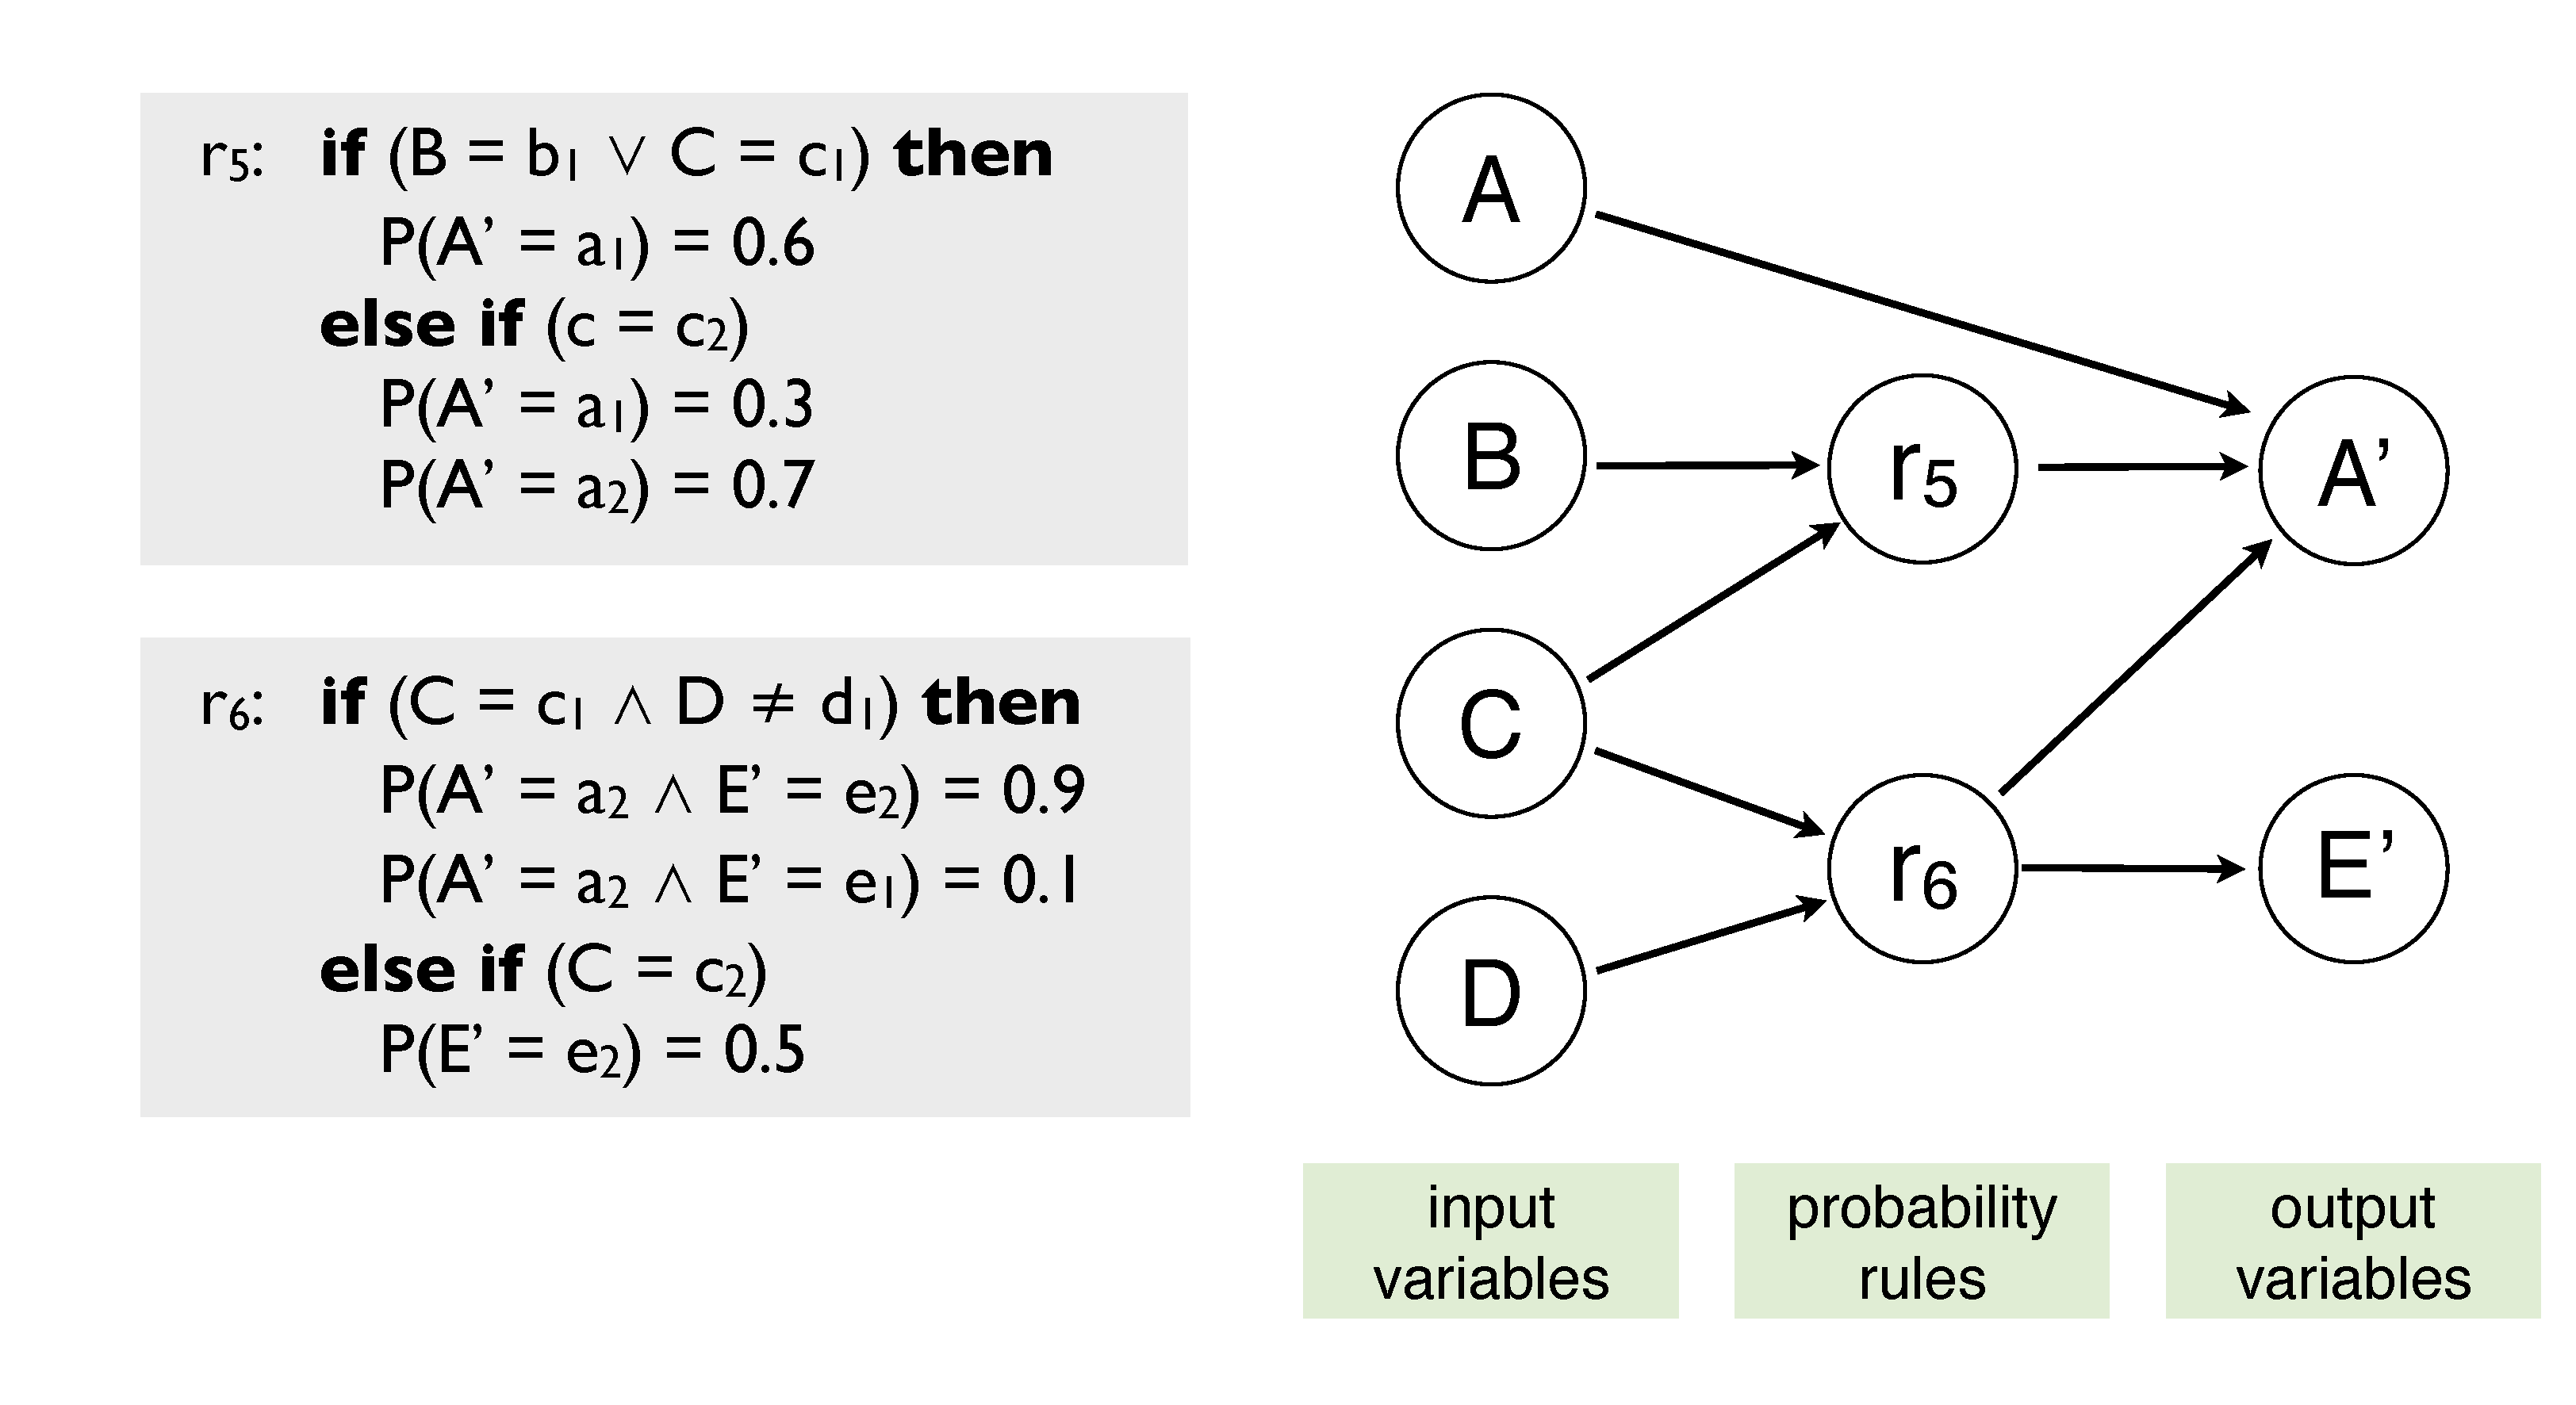
\includegraphics[scale=0.25]{imgs/ruleinstantiation.pdf}
\caption{Example of instantiation for the two probability rules $r_5$ and $r_6$. }
\label{fig:instantiationprob}
\end{figure}

The random variable represented by the node $r_5$ has three possible values that correspond to the three effects described in the rule: $\mathit{Val}(r_5) = \{ \{A'\!=\!a_1\}, \{A'\!=\!a_2\}, \{\cdot\}\}$, where $\{\cdot\}$ denotes the empty effect.  Similarly, the random variable $r_5$ has four alternative effects: $\mathit{Val}(r_6) = \{\{A'\!=\!a_2 \land E'\!=\!e_2\}, \{A'\!=\!a_2 \land E'\!=\!e_1\}, \{E'=e_2\}, \{\cdot\}\}$. 

We shall adopt the following terminology to denote the probability distributions created through the instantiation procedure: 
\begin{itemize}
\item The conditional probability distribution associated with rule nodes such as $r_5$ and $r_6$ given their inputs is a \textit{rule distribution}.
\item The conditional probability distribution associated with output variables such $A'$ and $E'$ given the rule nodes that determine it is an \textit{output distribution}.
\end{itemize}

\subsubsection*{Rule distributions}
\index{rule distribution}

The rule distributions directly reflect the rule semantics.  Formally, the conditional probability distribution of a rule node $r$ given its input variables $I_1, \dots, I_k$ is defined as: 
\begin{align}
& P(r\!=\!e \, | \, I_1\!=\!i_1, \dots, I_k\!=\!i_k) = P(E_i = e) \label{eq:ruledistrib}
 \\ 
& \; \; \; \; \; \; \; \; \text{ where } i = \min_i (c_i \text{ is satisfied with } I_1\!=\!i_1 \land \dots \land I_k\!=\!i_k) \nonumber 
\end{align}
Formally speaking, a condition $c_i$ is said to be satisfied iff the input assignment logically entails that the condition is true, that is: $(I_1\!=\!i_1 \land \dots \land I_k\!=\!i_k) \vdash c_i$. The rule conditions are checked in sequential order until one condition is found to be satisfied. As the last condition $c_n$ corresponds to the final \textbf{else} block and is therefore always trivially true, there will always be at least one satisfied condition. Once the first satisfied condition $c_i$ is found, the rule distribution is determined as the effect distribution $P(E_i\!=\!e)$.

As an example, the rule distribution $P(r_5 \, | \, B\!=\!b_1, C\!=\!c_1)$ for the node $r_5$ in Figure \ref{fig:instantiationprob} is straightforwardly defined as:
\begin{itemize}
\item $P(r_5 = \{A'\!=\!a_1\} \, | \, B\!=\!b_1, C\!=\!c_1) = 0.6$
\item  $P(r_5 = \{\cdot\} \, | \, B\!=\!b_1, C\!=\!c_1) = 0.4$
%\item $P(r_5 = \{A\!=\!a_2\} \, | \, B\!=\!b_1, C\!=\!c_1) = 0$
\end{itemize}

Similarly, the distribution $P(r_6 \, | \, C\!=\!c_1, D\!=\!d_1)$ is a distribution with the empty effect $\{\cdot\}$ assigned to a probability 1. 

\subsubsection*{Output distributions} 
\index{output distribution}

An output node $X'$ is conditionally dependent on all the rule nodes that refer to it in their effects.  In addition, output nodes that correspond to the updated version of existing nodes (such as $A'$ in the example of Figure \ref{fig:instantiationprob}) also include a conditional dependence on these existing nodes.

The output distribution is a reflection of the combination of effects specified in the parent rules. The conditional probability distribution $P(X'|r_1\!=\!e_1, \dots, r_n\!=\!e_n)$ for an output variable $X'$ with $n$ incoming rule nodes is defined in the following manner:
\begin{align}
&P(X'\!=\!x' \, | \, r_1\!=\!e_1, \dots, r_n\!=\!e_n) = \begin{dcases}
\frac{\mathbf{1}(x' \in {\mathbf{e}(X')})} { |\mathbf{e}(X')| } & \text{if } \mathbf{e}(X')\!\neq\!\emptyset \\
\mathbf{1}(x' = \mathit{None}) & \text{otherwise}
\end{dcases}
\label{eq:outputdist1}
\end{align}
where the following notation is used: \begin{itemize}
\item $\mathbf{e}$ is the conjunction of all effects, i.e.\ $\mathbf{e} = e_1 \land \dots \land e_n$.  This conjunction can include more than one assigned value for a particular variable.
\item $\mathbf{e}(X')$ denotes the (possibly empty) list of values specified for the variable $X'$ in $\mathbf{e}$. 
\item $\mathbf{1}(b)$ is the indicator function for a boolean $b$, with $\mathbf{1}(b)=1$ if $b$ is true and $0$ otherwise.
\end{itemize}

Equation \eqref{eq:outputdist1} stipulates that the distribution for $X'$ will follow the values assigned in the effect(s) provided that at least one effect specifies a value for it. If the effects include conflicting assignments, the distribution is spread uniformly over the alternative values. This uniform division of the probability mass reflects that, in the absence of further knowledge, all rules are assumed to have the same ``weight''. If two or more rules generate contradictory effects, there is therefore no way to tell which rule is to take precedence.\footnote{This assumption could, however, be refined in the future by e.g.\ associating numerical weights to particular rules or specifying a dominance hierarchy between the rules.} If no effects $e_1, \dots, e_n$ specifies a value for $X'$ , its value is set to a default $None$ value with probability 1. 

If the node $X'$ is an update of an existing node $X$, the procedure remains essentially the same as for Equation \eqref{eq:outputdist1}, except when all the effects specify empty assignments for the variable. In such a case, the distribution for $X'$ will fall back to the value defined for the existing node $X$ instead of being assigned a $\mathit{None}$ value:
\begin{align}
&P(X'\!=\!x' \, | \, r_1\!=\!e_1, \dots, r_n\!=\!e_n, X\!=\!x) = \begin{dcases} 
\frac{\mathbf{1}(x' \in {\mathbf{e}(X')})} { |\mathbf{e}(X')| }  & \text{if } \mathbf{e}(X')\!\neq\!\emptyset \\
\mathbf{1}(x' = x) & \text{otherwise}
\end{dcases}\label{eq:outputdist2}
\end{align}

As an example, the output distribution $P(A' \, | \, r_5\!=\!\{\cdot\},r_6\!=\!\{A'\!=\!a_2 \land E'\!=\!e_2\}, A\!=\!a_3)$ in Figure \ref{fig:instantiationprob} results in a deterministic distribution with a unique value $a_2$ with probability 1, since $\mathbf{e}(A') = \{a_2\}$. If the two rules generate conflicting assignments, the probability mass is divided equally over the alternative values.   The output distribution $P(A' \, | \, r_5\!=\!\{A'\!=\!a_1\},r_6\!=\!\{A'\!=\!a_2 \land E'\!=\!e_2\}, A\!=\!a_3)$ provides two alternative values for $A'$, since $\mathbf{e}(A')$ equates to $\{a_1,a_2\}$. The output distribution is thus in this case equivalent to a discrete uniform distribution with two values: $a_1$ and $a_2$, each with probability 0.5. Finally, if all effects are void, the output distribution is a simple copy of the distribution for the existing variable: $P(A' \, | \, r_5\!=\!\{\cdot\},r_6\!=\!\{\cdot\}, A\!=\!a_3)$ has a unique value $a_3$ with probability 1. 

%Output distributions are directly derived from the definition of effects in the rule nodes and are thus entirely parameter-free.  The ordering of the parent rules in the conditional probability distribution is arbitrary. %The resulting distribution bears resemblance to the probabilistic Independence of Causal Influence (pICI) described by \cite{diez06}. 


\subsubsection*{Instantiation algorithm} 
\label{sec:utilruleinstantiation}

The procedure for instantiating a rule in a given dialogue state is detailed in Algorithm \ref{algo:instantiateProbRule}. 

\begin{algorithm}[h!]
\caption{: \textsc{InstantiateProbRule} ($\mathcal{B}, \mathit{r}$)}
\begin{algorithmic}[1] \vspace{1mm}
\REQUIRE Bayesian network $\mathcal{B}$ for the current state
\REQUIRE Probability rule $\mathit{r}$ to instantiate in network  \vspace{1mm}
\STATE $I_1, \dots, I_k \leftarrow$ input variables for $\mathit{r}$
\STATE Create chance node $r$ with the rule distribution in Eq. \eqref{eq:ruledistrib}
\STATE Add node $r$ and dependency edges $I_1, \dots, I_k \rightarrow r$ to $\mathcal{B}$ 
\IF {$\mathit{Val}(r) = \{\cdot\}$}
\STATE Prune $r$ from $\mathcal{B}$
\ELSE
\STATE $O_1', \dots, O_l' \leftarrow$ output variables mentioned in the effects of $r$
\FORALL {variable $O' \in O_1', \dots, O_l'$}
\IF {$O'$ not already in $\mathcal{B}$}
\STATE Create chance node $O'$ with the output distribution in Eq. \eqref{eq:outputdist1}-\eqref{eq:outputdist2}
\STATE Add node $O'$ and (in case $O$ exists) dependency edge $O \rightarrow O'$ to $\mathcal{B}$
\ENDIF
\STATE Add dependency edge $r \rightarrow O'$ to $\mathcal{B}$ 
\ENDFOR
\ENDIF
\end{algorithmic}
\label{algo:instantiateProbRule}
\end{algorithm}

The first steps of the instantiation process are to extract in the Bayesian network the input variables of the rule (line 1), create a node corresponding to the rule (line 2) and include its dependency edges in the network (line 3).  The algorithm then checks whether at least one effect in $r$ is non-empty given its conditional dependencies (lines 4).  If all effects are empty, the rule node is irrelevant and can be directly pruned (line 5). Otherwise, the output variables are extracted (line 7), and output nodes that do not already exist in the network are created (line 10-11). The final step is to establish dependency edges between the rule node and these output variables (line 13).


\subsection{Utility rules}
\index{utility rule!instantiation of}

Utility rules are instantiated in the Bayesian network according to a similar procedure, with two notable differences compared to probability rules: \begin{itemize}
\item As utility rules define utility distributions, their instantiation corresponds to utility nodes instead of chance nodes.
\item Instead of output nodes, utility rules lead to the creation of new decision nodes. The dependency direction is inverted, as the decision node must be input to the utility node.
\end{itemize} 

The result of the instantiation process is a decision network that incorporates chance nodes (corresponding to the state variables), utility nodes (corresponding to the utility rules) and associated decision nodes. Figure \ref{fig:instantitionutil} illustrates the instantiation of two utility rules $r_7$ and $r_8$. 

\begin{figure}[ht]
\centering
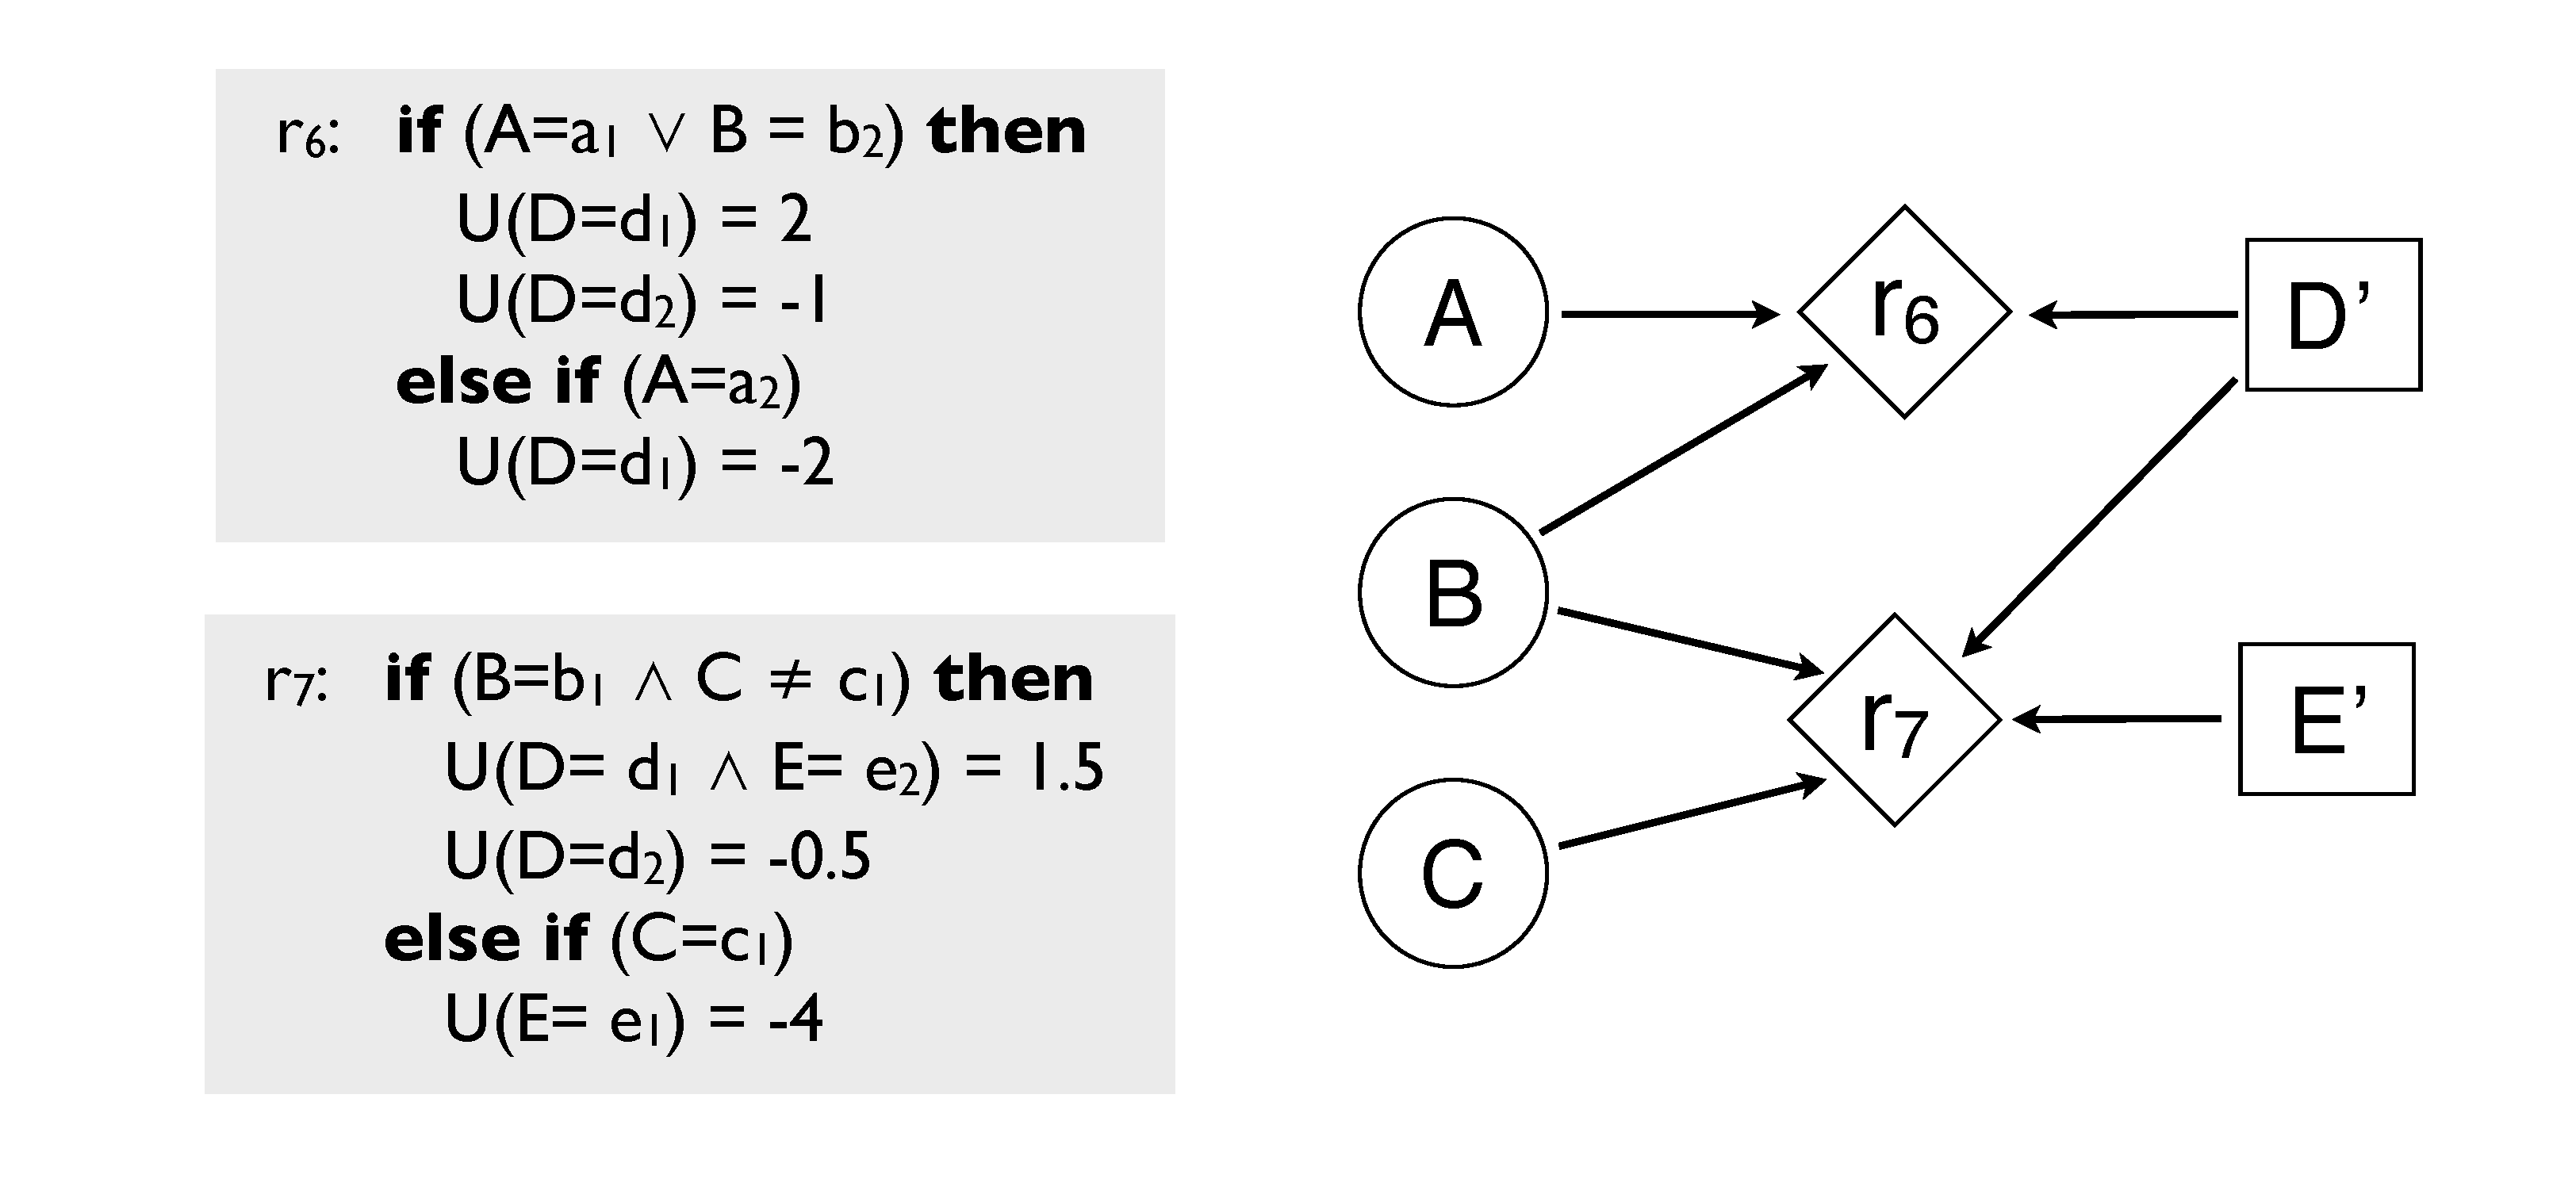
\includegraphics[scale=0.25]{imgs/ruleinstantiation2.pdf}
\caption{Example of instantiation for the two utility rules $r_7$ and $r_8$.}
\label{fig:instantitionutil}
\end{figure}

The utility distribution associated with each rule is a direct translation of the  \textit{if...then...else} rule.  Formally, the utility distribution generated by a rule $r$ with input variables $I_1, \dots, I_k$ and decision variables $D_1', \dots, D_l'$ is defined as:
\begin{align}
& U_r(D_1'\!=\!d_1, \dots, D_l'\!=\!d_l, I_1\!=\!i_1, \dots, I_k\!=\!i_k) = U_i(D_1'\!=\!d_1 \land \dots \land D_l'\!=\!d_l) \label{eq:utildistrib}\\
&  \; \; \; \; \; \; \; \;  \; \; \; \text{ where } i = \min_i (c_i \text{ is satisfied with } I_1\!=\!i_1 \land \dots \land I_k\!=\!i_k) \nonumber
\end{align}

If no utility is explicitly specified for $D_1'\!=\!d_1 \land \dots \land D_l'\!=\!d_l$ in the utility table, the default value is zero. 

As is conventionally assumed in decision networks, the total utility for a given assignment of decision variables is defined as the \textit{sum} of all utilities.  On the example of Figure \ref{fig:instantitionutil}, we can therefore calculate the total utility for the actions $D'\!=\!d_1 \ \land \ E'\!=\!e_1$ when $A\!=\!a_1$, $B\!=\!b_1$ and $C\!=\!c_1$ to be equal to $2 - 4 = -2$. 


\subsubsection*{Instantiation algorithm} 

The procedure for instantiating a utility rule is similar to the one already outlined for probability rules. Algorithm \ref{algo:instantiateUtilRule} details the procedure, starting from the extraction of the input variables, the creation of the rule node, and the inclusion of conditional dependencies (line 1-3). The algorithm then checks if the utility distribution stipulates a non-zero utility for at least one decision (line 4).  If the answer is negative, the node is essentially irrelevant and can be pruned (line 5).  The decision variables associated with the rule are extracted (line 7), and a corresponding decision node is created if it does not already exist (line 10). Finally, the possible values specified for the decision variable are integrated to the node (line 12), and a dependency edge is established between the decision node and the utility node for the rule (line 13). 

\begin{algorithm}[h!]
\caption{: \textsc{InstantiateUtilRule} ($\mathcal{B}, \mathit{r}$)}
\begin{algorithmic}[1] \vspace{1mm}
\REQUIRE Bayesian network $\mathcal{B}$ for the current state
\REQUIRE Utility rule $\mathit{r}$ to instantiate in network  \vspace{1mm}
\STATE $I_1, \dots, I_k \leftarrow $ input variables for $r$
\STATE Create utility node $r$ with the utility distribution in Eq. \eqref{eq:utildistrib}
\STATE Add node $r$ and dependency edges $I_1, \dots, I_k \rightarrow r$ to $\mathcal{B}$ 
\IF {utility distribution is empty for all inputs}
\STATE Prune $r$ from $\mathcal{B}$
\ELSE
\STATE $D_1', \dots, D_l' \leftarrow$ decision variables mentioned in the effects of $r$
\FORALL {variable $D' \in D_1', \dots, D_l'$}
\IF {$D'$ not already in $\mathcal{B}$}
\STATE Create decision node $D'$ and add it to $\mathcal{B}$
\ENDIF
\STATE Add in $\mathit{Val}(D')$ the action values specified in the effects of $r$
\STATE Add dependency edge $D' \rightarrow r$ to $\mathcal{B}$ 
\ENDFOR
\ENDIF
\end{algorithmic}
\label{algo:instantiateUtilRule}
\end{algorithm}

\subsection{Quantification}
\label{sec:applicationquantif}
\index{probabilistic rule!quantifiers in}

We saw in Section \ref{sec:quantification} that conditions and effects could include universally quantified variables, but have not yet discussed how such underspecified rules could be practically instantiated in the Bayesian network. The general instantiation principle remains unchanged: To each rule corresponds a distinct rule node responsible for the mapping between input and output variables (or decision variables for utility rules). The instantiation procedure must nevertheless be extended to accommodate the presence of quantified variables.  The key idea is to find all relevant \textit{groundings} for the quantified variables, and then calculate the effect distribution for each grounding. This method of handling quantifiers by extracting all possible groundings and reasoning at the propositional level is an instance of \textit{ground inference}\index{ground inference} \citep{getoor:srlbook07}. 

\subsubsection*{Extraction of input variables}

Universally quantified rules may underspecify both the names and values of random variables, as we saw in the examples of Section \ref{sec:quantification}.  Rule $r_3$ includes for instance a reference to an underspecified random variable $\mathit{shape}(y)$.  In order to instantiate the rule, the system must therefore first determine the set of all random variables in the current state that match the underspecified description, as these variables should be included in the conditional dependencies of the rule node. 

In practice, this extraction of input variables is simply achieved by looping over all current state variables and searching for those that may offer a potential match for at least one underspecified description. If rule $r_3$ is instantiated in a state containing two objects $o_1$ and $o_2$ (each with a specific shape), the resulting input variables will be $\mathit{shape}(o_1)$ and $\mathit{shape}(o_2)$. 

%Algorithm \ref{algo:getinputvariables} outlines how this search for matching input variables can proceed. The first step is to extract the initial input variables associated with the rule, which may include underspecified descriptions such as $\mathit{shape}(y)$. The algorithm then loops on each underspecified description to find possible groundings in the random variables of the Bayesian network.  The final result corresponds to the union of the fully specified input variables and the set of possible groundings for the underspecified variables.  

%\begin{algorithm}[h!]
%\caption{: \textsc{GetInputVariables} ($\mathcal{B}, \mathit{r}$)}
%\begin{algorithmic}[1] \vspace{1mm}
%\REQUIRE Bayesian network $\mathcal{B}$ for the current state
%\REQUIRE Probability or utility rule $\mathit{r}$ \vspace{1mm}
%\STATE $\mathcal{I}_{r} \leftarrow $ Initial (possibly underspecified) input variables for $\mathit{r}$
%\STATE $\mathcal{U}_{r} \leftarrow $ Subset of variable names in $\mathcal{I}_{r}$ that are underspecified
%\STATE $\mathcal{G}_{r} \leftarrow$ Set of possible groundings for $\mathcal{U}_{r}$, initially empty
%\FOR {underspecified variable name $u \in \mathcal{U}_{r}$}
%\FOR {random variable $X$ in $\mathcal{B}$}
%\IF {$X$ matches $u$}
%\STATE $\mathcal{G}_{r} \leftarrow \mathcal{G}_{r} \cup [X]$
%\ENDIF
%\ENDFOR
%\ENDFOR
%\RETURN $(\mathcal{I}_{r} \ / \ \mathcal{U}_{r}) \ \cup \  \mathcal{G}_{r}$
%\end{algorithmic}
%\label{algo:getinputvariables}
%\end{algorithm}

 %Line 1 in Algorithms \ref{algo:instantiateProbRule} and \ref{algo:instantiateUtilRule} is then replaced by: 
%\begin{algorithmic}[1] \vspace{1mm}
%\STATE $I_1,...I_k \leftarrow $ \textsc{GetInputVariables} ($\mathcal{B}, \mathit{r}$)
%\end{algorithmic}


\subsubsection*{Extraction of relevant groundings}
\index{probabilistic rule!grounding of}

Once the input variables are retrieved, the next step is to establish the set of relevant groundings for the universally quantified variables in the rule.  The groundings are always determined relative to a particular assignment of values for the (grounded) input variables $I_1, \dots, I_k$. 

Given a particular input assignment $I_1\!=\!i_1 \land \dots \land I_k\!=\!i_k$, the set of groundings is derived by extracting the ground terms (constants and functions of constants) from the input assignment that can function as proper substitutions for the universally quantified variables. At the end of the extraction procedure, the universally quantified variables of the rule will therefore be associated with a set of possible groundings $G = \{\mathbf{g}_1, \dots, \mathbf{g}_{|G|}\}$.  For instance, the rule $r_3$ and the input assignment $ \mathit{shape}(o_1)\!=\!\mathit{sphere} \land \mathit{shape}(o_2)\!=\!\mathit{cone}$ yields the groundings $G= \{[o_1], [o_2]\}$ for the variable $y$. 

% These ground terms define the domain of discourse for these variables. 

\subsubsection*{Quantified probability rules}
\index{probability rule!quantifiers in}

As we have seen, probability rules are instantiated as chance nodes associated with a rule distribution.  For rules including universal quantifiers, each grounding in $G$ gives rise to a particular distribution over effects.   We can define a grounding-specific rule distribution where the universally quantified variables $\mathbf{y} = y_1,..., y_p$ are replaced by a specific grounding $\mathbf{g}_j$:
\begin{align}
& P(r_{\mathbf{g}_j}\!=\!e [\mathbf{y} / \mathbf{g}_j] \, | \, I_1\!=\!i_1, \dots, I_k\!=\!i_k) = P(E_i = e) \label{eq:quantifruledistrib}
 \\
& \; \; \; \; \; \; \; \; \text{where } i = \min_i (c_i[\mathbf{y} / \mathbf{g}_j]\text{ is satisfied with } I_1\!=\!i_1 \land \dots \land I_k\!=\!i_k) \nonumber \end{align}

The expression $\phi[a/b]$ denotes (as in formal logic) the formula $\phi$ where all instances of $a$ are substituted by $b$. The rule distribution in Equation \eqref{eq:quantifruledistrib} is thus identical to Equation \eqref{eq:ruledistrib} where all occurrences of the universally quantified variables in the conditions and effects are replaced by their grounded value in $\mathbf{g}_j$.

The procedure results in a set of grounding-specific rule distributions $ \{ P(r_{\mathbf{g}_1}), \dots, P(r_{\mathbf{g}_{|G|}}) \}$. Empty and redundant effect distributions are discarded. The final probability distribution for the rule node is then defined as the joint distribution over these grounding-specific distributions: 
\begin{align}
& P(r\!=\![e_1 \land \dots \land e_{|G|}] \, | \, I_1\!=\!i_1, \dots, I_k\!=\!i_k) = \prod_{j=1}^{|G|} P(r_{\mathbf{g}_j}\!=\!e_j) \label{eq:quantifruledistrib2}
\end{align}


Figure \ref{fig:quantinstantitionprob} shows the instantiation of the rule $r_3$ in a state with two objects $o_1$ and $o_2$, each associated with a random variable describing its shape. The effects specified for $r_3$ have two output variables: $\mathit{graspable}'(o_1)$ and $\mathit{graspable}'(o_2)$ which are thus placed as children of the node $r_3$.  

\begin{figure}[ht]
\centering
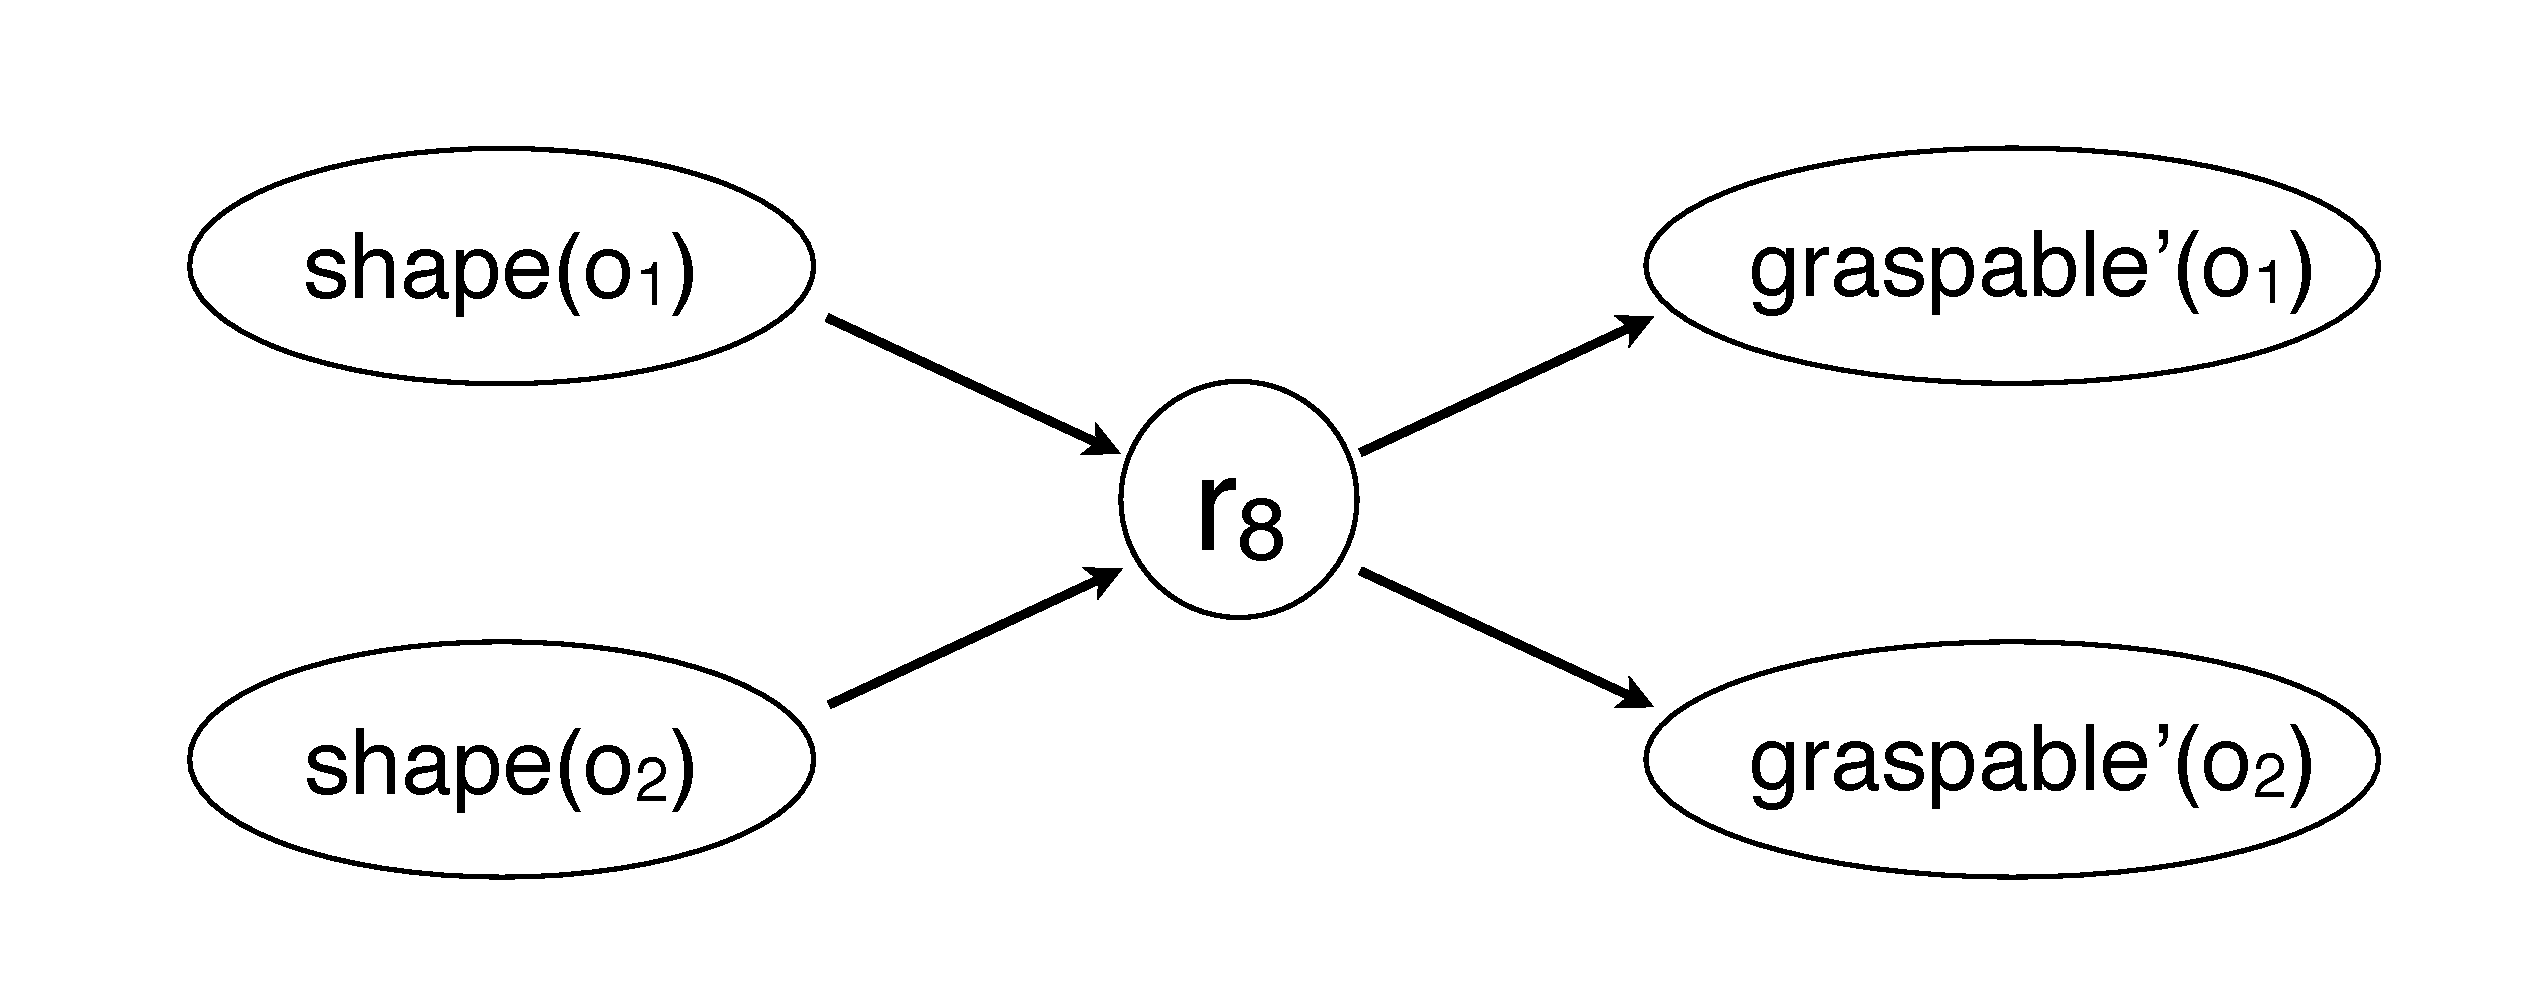
\includegraphics[scale=0.25]{imgs/quantruleinstantiation.pdf}
\caption{Instantiation of the probability rule $r_3$ on a state with two objects $o_1$ and $o_2$.}
\label{fig:quantinstantitionprob}
\end{figure}

To illustrate the application of Equations \eqref{eq:quantifruledistrib} and \eqref{eq:quantifruledistrib2}, the probability distribution $P(r_3 \, | \, \mathit{shape}(o_1)\!=\!\mathit{sphere}, \mathit{shape}(o_2)\!=\!\mathit{cone})$ has two relevant groundings $y\!=\!o_1$ and $y\!=\!o_2$, from which we derive four effects:
\begin{itemize}
\item $\{\mathit{graspable}(o_1)'\!=\!true \land \mathit{graspable}(o_2)'\!=\!true \} $ with probability $0.9\times0.2\!=\!0.18$
\item $\{\mathit{graspable}(o_1)'\!=\!true \ \land \  \mathit{graspable}(o_2)'\!=\!false\}$ with probability $0.9\times0.8\!=\!0.72$ 
\item $\{ \mathit{graspable}(o_1)'\!=\!false \land \mathit{graspable}(o_2)'\!=\!true \}$ with probability $0.1\times0.2\!=\!0.02$
\item $\{\mathit{graspable}(o_1)'\!=\!false \land \mathit{graspable}(o_2)'\!=\!false\}$ with probability $0.1\times0.8\!=\!0.08$
\end{itemize}


\subsubsection*{Quantified utility rules}
\index{utility rule!quantifiers in}

Utility rules are similarly extended to accommodate universally quantified variables. As for probability rules, the instantiation of utility rules proceeds by determining a set of groundings and generating a particular utility distribution for each. 
For a utility rule $r$ with input variables $I_1, \dots, I_k$ and decision variables $D_1', \dots, D_l'$, the rule utility for the grounding $\mathbf{g}_j$ is defined as:
 \begin{align}
& U_{\mathbf{g}_j}(D_1'\!=\!d_1[\mathbf{y} / \mathbf{g}_j], \dots, D_l'\!=\!d_l[\mathbf{y} / \mathbf{g}_j], I_1\!=\!i_1, \dots, I_k\!=\!i_k) \label{eq:quantifuruledistrib} \\ 
& \; \; \; \; \; \; \; \;   \; \; = U_i(D_1'\!=\!d_1 \land \dots \land D_l'\!=\!d_l) \nonumber \\
& \; \; \; \; \; \; \; \;   \; \; \;\text{where } i = \min_i (c_i[\mathbf{y} / \mathbf{g}_j]\text{ is satisfied with } I_1\!=\!i_1 \land \dots \land I_k\!=\!i_k) \nonumber
\end{align}

After discarding empty and redundant distributions, the result is a set of utility distributions $ \{ U_{\mathbf{g}_1}, \dots, U_{\mathbf{g}_{|G|}} \}$. The total utility distribution for the rule $r$ is finally constructed by adding up the grounding-specific utility distributions:   
\begin{align}
& U_{r}(I_1, \dots, I_k, D_1'\, \dots, D_l') = \sum_{j=1}^{|G|} U_{\mathbf{g}_j}(I_1, \dots, I_k, D_1', \dots, D_l') \label{eq:quantifuruledistrib2}
\end{align}


The instantiation of rule $r_4$ given the input variables $\mathit{task}$, $\mathit{graspable}(o_1)$ and $\mathit{graspable}(o_2)$ is shown in Figure  \ref{fig:quantinstantitionutil}.  The utility distribution for the input assignment $\mathit{task}\!=\!\mathit{grasp}(o_1) \land \mathit{graspable}(o_1) \!=\!\mathit{true} \land \mathit{graspable}(o_2)\!=\!\mathit{false}$ assigns for instance the action $a_m'\!=\!\mathit{grasp}(o_1)$ to a utility of 2, while $a_m'\!=\!\mathit{grasp(o_2)}$ is assigned to a utility of -2 in this situation.

\begin{figure}[ht]
\centering
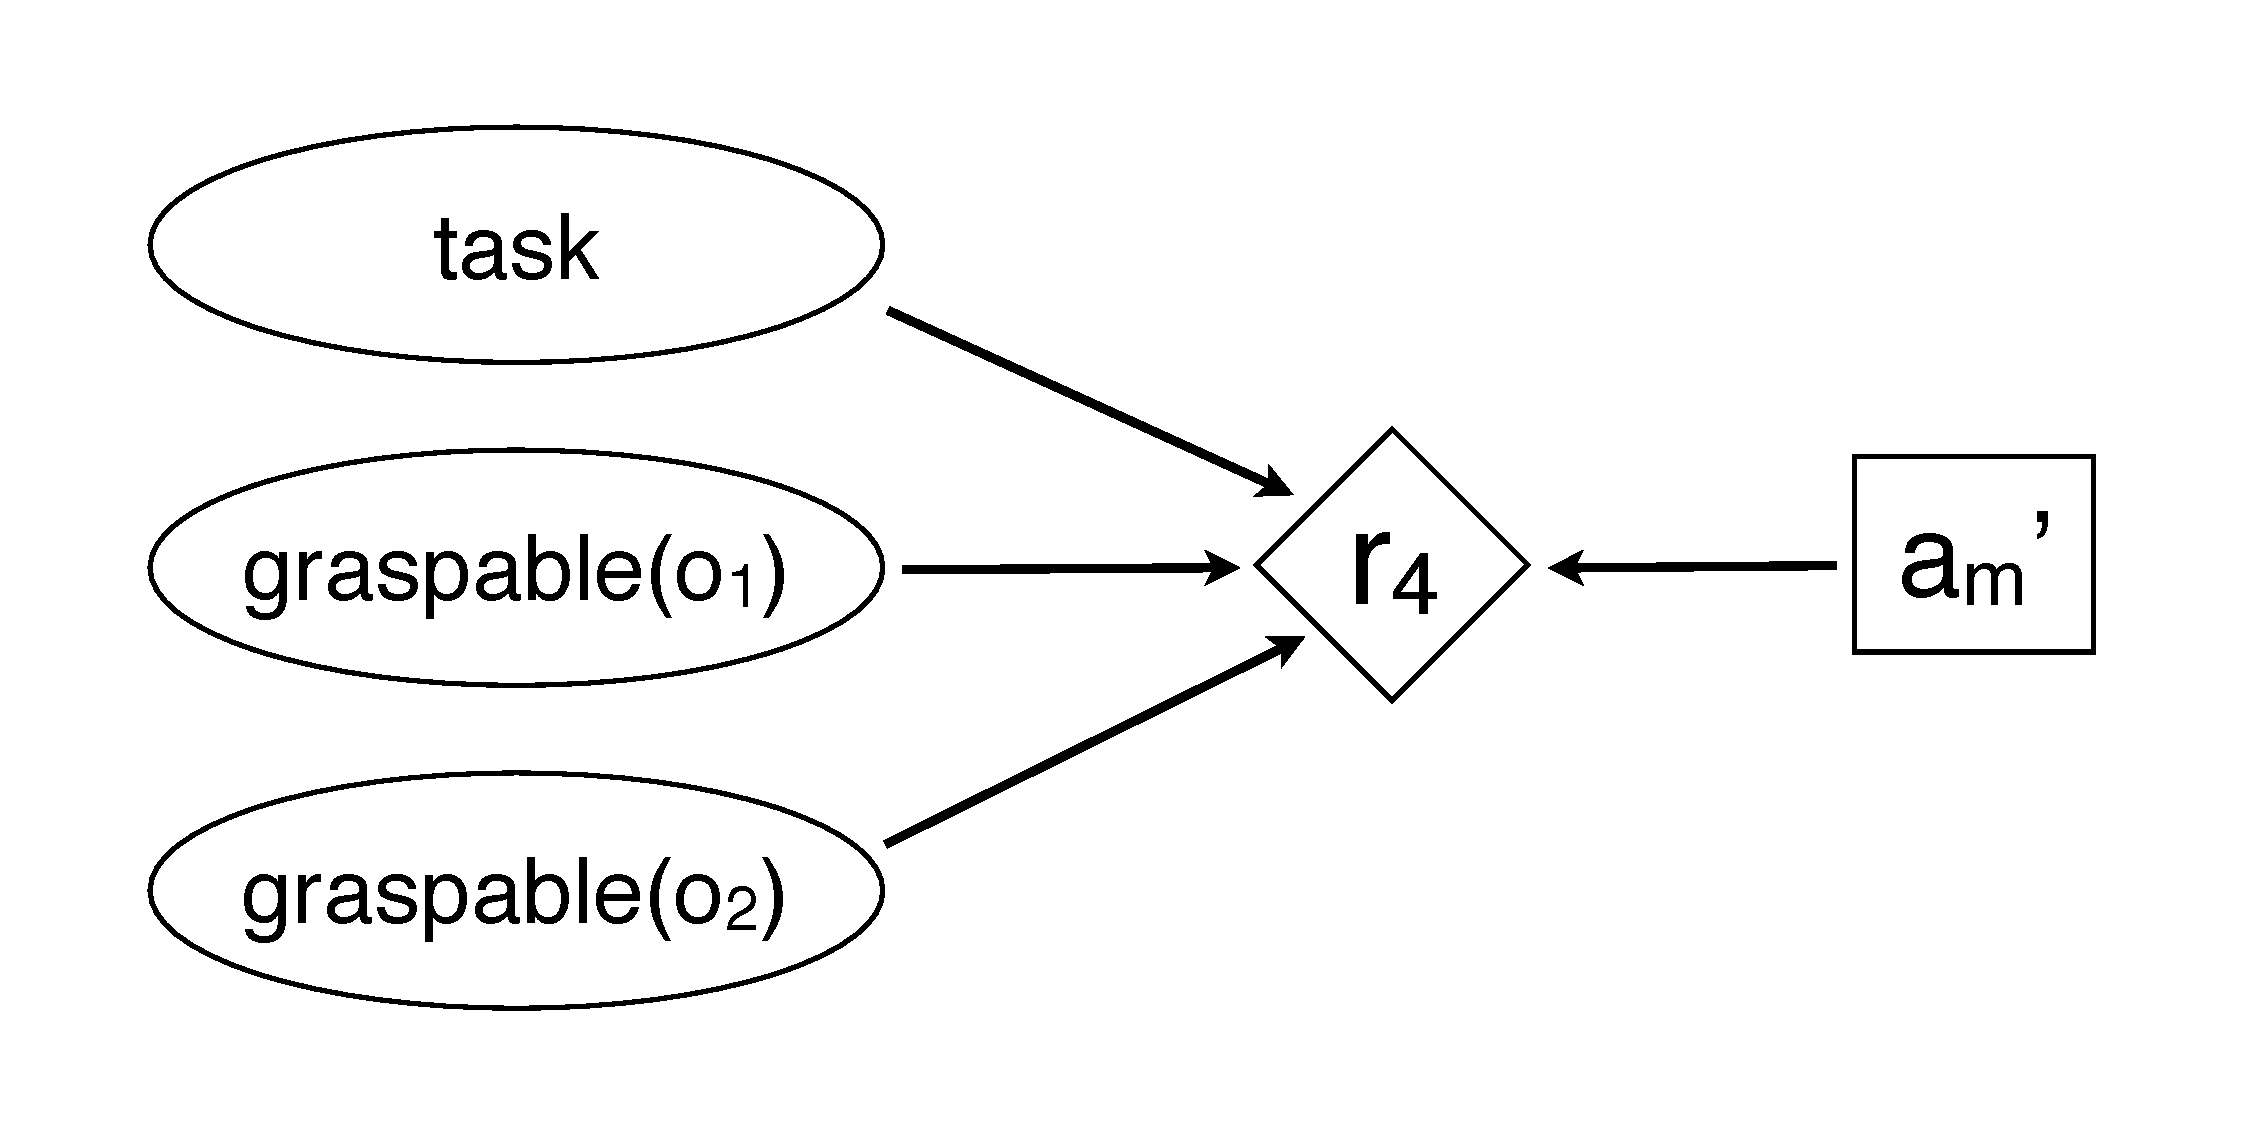
\includegraphics[scale=0.25]{imgs/quantutilruleinstantiation.pdf}
\caption{Instantiation of the quantified utility rule $r_9$ on a state with two objects $o_1$ and $o_2$.}
\label{fig:quantinstantitionutil}
\end{figure}

\subsubsection*{Tractability aspects}

Although the use of universal quantifiers can greatly improve the expressivity of probabilistic rules, they also tend to increase the in- and out-degrees of rule nodes (that is, the cardinality of their parents and children nodes). Approximate inference techniques are thus necessary to handle this conditional structure in a tractable manner. Sampling methods such as likelihood weighting (cf. Section \ref{sec:inference}) have in practice proved to work well in this setting.

The groundings are always extracted \textit{given a specific assignment of values} for the input variables. By restricting the groundings to this limited domain of discourse, we ensure that the number of grounding-specific distributions enumerated in Equations \eqref{eq:quantifruledistrib2} and \eqref{eq:quantifuruledistrib2} remains small.   This procedure was found to be much more efficient than copying the rule in distinct nodes, as investigated in earlier implementations of the formalism \citep{relational-apl2012}.  This procedure departs from other frameworks such as Markov logic networks, where the functions and predicates are duplicated for every possible grounding of variables in the domain \citep{Richardson:2006}.


 %In order to keep the number of groundings under control, the specification of probabilistic rules should nevertheless refrain from introducing more universally quantified variables than necessary.

%

\section{Processing workflow}
\label{sec:processing-workflow}
\index{dialogue state!update of}

The two previous sections detailed how probability and utility rules are internally defined, and how they can be instantiated as latent nodes of a graphical model. We are now ready to explain how collections of rules are practically applied at runtime to update the dialogue state and perform action selection. The general workflow is strongly inspired by information-state approaches to dialogue management \citep{Larsson:2000}, as the dialogue state serves as a central blackboard monitored by various groups of rules that are ``triggered'' upon relevant changes. 

The following section first describes how dialogue domains are organised in collections of rules that we call \textit{models}, and then goes on to explain how these models are applied to update state variables and express the utility of particular actions. We also demonstrate the general processing workflow on a detailed example. 


\subsection{Domain representation}

The specification of dialogue domains\index{dialogue domain} can comprise multiple probability and utility rules. These rules are internally grouped in collections of rules called \textit{models}\index{rule-structured model}. A model is simply a set of rules that is associated with one or more ``trigger'' variables that specify when the rules should be instantiated. Each model is attached to the dialogue state and monitors it to detect changes affecting its trigger variables. When at least one trigger variable is modified at runtime by another module, they lead to the instantiation of all rules included in the model. Formally, a model $m$ is defined as a pair $\langle \mathcal{T}_m, \mathcal{R}_m \rangle$ where $\mathcal{T}_m$ corresponds to the trigger variables and $\mathcal{R}_m$ to the rules in the model.  There is no restriction on the trigger variables $\mathcal{T}_m$ associated with each rule-structured model.  In particular, several models can share the same trigger variable(s) and be therefore triggered in parallel upon a given change in the dialogue state. 

A dialogue domain is represented as a pair $\langle \mathcal{B}_0, \mathcal{M} \rangle$, where $\mathcal{B}_0$ is the initial dialogue state  and $\mathcal{M}$ the set of models attached to it. The organisation of rules into models allows the system designer to structure the application pipeline in a modular manner. Each model can be intuitively viewed as a distinct component responsible for a particular inference or decision step. 

Section \ref{sec:domain-specification} explains how dialogue domains (and the models that compose them) are practically encoded in the \opendial{} architecture, based on an XML format. \index{openDial@\opendial{}}

\subsection{Update algorithm} 
\index{dialogue state!update of}

%The software architecture adopted in this thesis takes the form of an event-driven blackboard architecture revolving around a dialogue state $\mathcal{B}$ represented as a Bayesian network.  %As in information state approaches, this dialogue state functions as a central informational hub for the architecture and is continuously read and written by the system modules. 

The dialogue state is represented in our approach as a Bayesian network and is denoted $\mathcal{B}$. Each node in this Bayesian network represents a distinct state variable and can be connected to other variables through various conditional dependencies. As in information-state approaches to dialogue management, the dialogue state stands at the centre of the architecture and serves as a shared information repository for the whole dialogue system. 

The general procedure for updating this dialogue state upon the reception of new observations is shown in Algorithm \ref{algo:stateupdate}. The observations may for instance correspond to new user inputs processed by the ASR/NLU components or to new elements perceived in the external context. The first step is to insert the variables in the dialogue state (line 2). The algorithm then triggers the instantiation of the relevant domain models (line 3), leading to a chain of updates.  If the expanded dialogue state contains decision and utility variables, the algorithm searches for the optimal action, selects it, and activates the models that are triggered as a result (lines 5-7). Finally, the updated state is reduced by pruning away unnecessary nodes and incorporating the evidence (line 9). 

\begin{algorithm}[ht]
\caption{: \textsc{UpdateState} ($\mathcal{B}, \mathbf{O}$)}
\begin{algorithmic}[1] \vspace{1mm}
\REQUIRE Bayesian network $\mathcal{B}$ for the current state
\REQUIRE New observations $\mathbf{O}$ to insert in the state \vspace{1mm}
\STATE Initialise evidence $\mathbf{e} \leftarrow \emptyset$
\STATE $\mathcal{B}, \mathbf{e} \leftarrow $ \textsc{AddToState}($\mathcal{B}, \mathbf{e}, \mathbf{O}$)
\STATE $\mathcal{B}, \mathbf{e} \leftarrow$ \textsc{TriggerModels} ($\mathcal{B}, \mathbf{e},  \mathbf{O}$) \vspace{1mm}
\WHILE {$\mathcal{B}$ contains decision variables}
\STATE $\mathbf{a}^* \leftarrow $ \textsc{SelectAction} ($\mathcal{B}, \mathbf{e}$)
\STATE Assign $\mathbf{A}' = \mathbf{a}^*$
\STATE $\mathcal{B}, \mathbf{e} \leftarrow$ \textsc{TriggerModels} ($\mathcal{B}, \mathbf{e}, \mathbf{A}'$)
\ENDWHILE \vspace{1mm}
\STATE $\mathcal{B} \leftarrow \textsc{PruneState} (\mathcal{B}, \mathbf{e})$ \vspace{1mm}
\end{algorithmic}
\label{algo:stateupdate}
\end{algorithm}

We now describe each of these steps in detail.

\subsubsection*{Adding new observations to the state}

The first step in the update procedure is to add the new observation(s) into the dialogue state. Since dialogue domains often include predictions on variables that will be observed in the next time steps,\footnote{This is for instance the case for the user action model $P(a_u' \, | \, i_u', a_m)$, that estimates the relative probabilities for the next dialogue action from the user. The predictions provide a prior on the future observation of the user action.} these observations must be connected to their corresponding predicted values.

In order to distinguish random variables that express a prediction on a future outcome from those that reflect an actual (although possibly uncertain) observation, we denote all predictive variables with a superscript $p$. A variable $X^p$ thus represents a random variable on the predicted values of the variable $X$ to be observed in the future. 


\begin{wrapfigure}[12]{r}{48mm}
\vspace{-5mm}
\centering
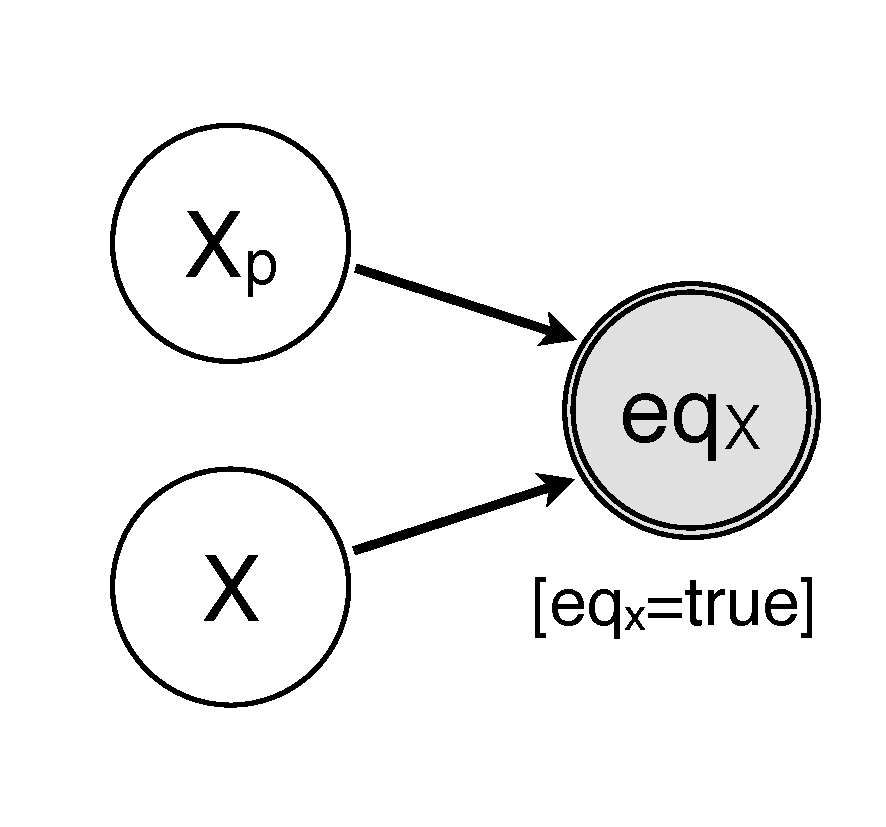
\includegraphics[scale=0.25]{imgs/prediction.pdf} 
\vspace{-2mm}
\caption{Equivalence node $\mathit{eq}_{X}$ with parents $X$ and $X^p$ (the double circle denotes a deterministic distribution).}
\label{fig:prediction}
\end{wrapfigure}

Prediction and observation variables must be related with one another at runtime.  In the case where the observation is known with certainty, this relation can simply take the form of an assignment of evidence values.  However, dialogue domains often include observations that are themselves uncertain and represent ``soft'' or virtual evidence\index{soft evidence}.  Several techniques are available to practically encode such kind of evidence \citep{Pan06beliefupdate}. The method adopted in this thesis is to add a new boolean-valued chance node, subsequently called the \textit{equivalence node}\index{equivalence node} $\mathit{eq}_{X}$, that is conditionally dependent on both $X$ and $X^p$, as shown in Figure \ref{fig:prediction}. The use of a distinct node to express the evidence is motivated by the fact that $X$ and $X^p$ may have arbitrary incoming and outgoing edges with other variables. 

The conditional probability distribution for $\mathit{eq}_X$ given $X$ and $X^p$ is deterministic:
\begin{equation}
P(\mathit{eq}_{X}\!=\!true \, | \, X\!=\!x, X^p\!=\!x^p) = \begin{cases}
1 & \text{if } x = x^p \\
0 & \text{otherwise}
\end{cases} \label{eq:equivdistrib}
\end{equation}

The assignment $\mathit{eq}_{X} \!=\! true$ is added to the evidence. The posterior distribution given the evidence allows the prediction to act as a prior for the observed distribution:
\begin{align}
&P(X = x \, | \, \mathit{eq}_{X}\!=\!true) \nonumber \\
&=  \eta \ P(X\!=\!x)  \sum_{x^p \in \mathit{Val}(X^p)} P(\mathit{eq}_{X}\!=\!true\, |\, X\!=\!x, X^p \!=\!x^p ) P(X^p\!=\!x^p)  \nonumber\\
&= \eta \ P(X\!=\!x) \ P(X^p\!=\!x)  \nonumber 
\end{align}

%The inclusion of an equivalence node between $X$ and $X^p$ with evidence  $[\mathit{eq}_{X}\!=\!true]$ modifies the distribution of the variables $X$ and$X^p$ as well as their respective parents and children. 

Algorithm \ref{algo:AddToState} details how the insertion of new observation variables $\mathit{ObsVars}$ into the dialogue state is performed in practice. 

\begin{algorithm}[ht]
\caption{: \textsc{AddToState} ($\mathcal{B}, \mathbf{e}, \mathit{ObsVars}$)}
\begin{algorithmic}[1] \vspace{1mm}
\FORALL {$X \in \mathit{ObsVars}$}
\IF {$X \notin \mathcal{B}$}
\STATE Insert $X$ in $\mathcal{B}$ 
\ENDIF
\IF {there is a corresponding prediction variable $X^p \in \mathcal{B}$}
\STATE Create equivalence node $\mathit{eq}_{X}$ with distribution in Eq. \eqref{eq:equivdistrib}
\STATE Insert $\mathit{eq}_{X}$ in $\mathcal{B}$ with parents $\mathit{X}$ and $\mathit{X}^p$
\STATE Add assignment $[\mathit{eq}_{X}\!=\!true]$ to evidence $\mathbf{e}$
\ENDIF
\ENDFOR
\RETURN $\mathcal{B}, \mathbf{e}$
\end{algorithmic}
\label{algo:AddToState}
\end{algorithm}



\subsubsection*{Model instantiation}
\index{rule-structured model!instantiation of}

After inserting the new variables in the dialogue state and connecting them to their predicted values, the next step in the processing workflow is to trigger the relevant rule-structured models. 

Algorithm \ref{algo:triggerModels} summarises the steps involved in the instantiation of the models. The algorithm takes three arguments: a dialogue state $\mathcal{B}$ represented as a Bayesian network, an assignment of evidence values and a list of random variables that have been recently updated in the dialogue state. The algorithm loops on all domain models and instantiates the ones that are triggered by the updated variables. The rules are instantiated one by one, following the procedure we have outlined in the previous section. Once all models are traversed, the output variables of the instantiated rules become updated variables themselves, and the procedure is repeated until no more models can be applied.  To avoid the occurrence of infinite triggering cycles, models are limited to one single instantiation per update. The algorithm returns both the dialogue state expanded with new variables, and the evidence assignments attached to the equivalence nodes. 


\begin{algorithm}[t]
\caption{: \textsc{TriggerModels} ($\mathcal{B}, \mathbf{e}, \mathit{UpdatedVars}$)}
\begin{algorithmic}[1] \vspace{1mm}
\WHILE {$\mathit{UpdatedVars} \neq \emptyset$}
\STATE $\mathit{NewVars} \leftarrow \emptyset$
\FORALL {models $m$}
\IF {$(\mathit{UpdatedVars} \cap \mathcal{T}_m) \neq \emptyset$ and $m$ has not yet been applied}
\FORALL {rule $r \in \mathcal{R}_m$}
\IF {$r$ is a probability rule}
\STATE $\mathcal{B} \leftarrow \textsc{InstantiateProbRule}(\mathcal{B},r)$
\ELSIF {$r$ is a utility rule}
\STATE $\mathcal{B} \leftarrow \textsc{InstantiateUtilRule}(\mathcal{B},r)$
\ENDIF
\STATE Let $\mathcal{O}_r$ be the new output variables created by rule $r$
\STATE $\mathit{NewVars} \leftarrow \mathit{NewVars} \cup \mathcal{O}_r$
\STATE $\mathcal{B}, \mathbf{e} \leftarrow $ \textsc{AddToState}($\mathcal{B}, \mathbf{e}, \mathcal{O}_r)$
\ENDFOR
\ENDIF
\ENDFOR 
\STATE $\mathit{UpdatedVars} \leftarrow \mathit{NewVars}$
\ENDWHILE 
\RETURN $\mathcal{B}, \mathbf{e}$
\end{algorithmic}
\label{algo:triggerModels}
\end{algorithm}


\subsubsection*{Action selection}
\index{action selection}

Whenever the new dialogue state contains utility and decision nodes, the system must decide on the action to perform.  Algorithm \ref{algo:actionselection} illustrates how actions can be selected on the basis of the current dialogue state augmented with the decision and utility nodes created by the utility rules. The algorithm searches for the assignment of action values that maximise the current utility given the dialogue state and the evidence and returns it. This utility maximisation is based on standard inference algorithms for decision networks such as likelihood weighting (cf. Section \ref{sec:inference}). 

The utility nodes are removed from the state once the decision is made. The action selection procedure described in Algorithm \ref{algo:actionselection} only takes into account the current (immediate) utility and does not rely on forward planning.  Chapter \ref{chap:rllearning} demonstrates how this procedure can be extended to perform online planning on a limited horizon. 


\begin{algorithm}[h]
\caption{: \textsc{SelectAction} ($\mathcal{B}, \mathbf{e}$)}
\begin{algorithmic}[1] \vspace{1mm}
\STATE Let $\mathbf{A}'$ be the set of all decision variables in $\mathcal{B}$
\STATE Find optimal value $\mathbf{a}^* = \argmax_{\mathbf{a}} U(\mathbf{A}' = \mathbf{a}, \mathbf{e})$
\STATE Remove utility nodes from the state $\mathcal{B}$
\RETURN $\mathbf{a}^*$
\end{algorithmic}
\label{algo:actionselection}
\end{algorithm}

\subsubsection*{State pruning}
\index{dialogue state!pruning of}

The instantiation of the domain models results in the inclusion of numerous new nodes in the dialogue state. However, many nodes in this expanded Bayesian network  only serve as intermediaries and do not directly express meaningful information about the current state of the dialogue. The last step is therefore to reduce the dialogue state to its minimal size, by removing all intermediary nodes -- including rule nodes, outdated versions of state variables, equivalence nodes and predictive nodes that are attached to them -- in order to only retain current state variables. The accumulated evidence is also integrated in the posterior distribution of the state variables.

The procedure is outlined in Algorithm \ref{algo:pruneState}. The first step is to determine which nodes to keep (lines 1-6).  Only the most recent versions of state variables are retained. 
The nodes are then added one by one in a new dialogue state $\mathcal{B}'$.  The parents of the retained variables are determined, and their conditional probability distributions are calculated given the evidence.  The parents of a state variable are the closest ancestors of the variable within the subset of nodes in $\mathit{NodesToKeep}$, and its conditional probability distribution is determined as $P_{\mathcal{B}}(N \, | \, \mathit{Parents}, \mathbf{e})$.  This posterior distribution is calculated via sampling techniques. This is done by sampling all nodes in $\mathcal{B}$, then deriving the distributions $P_{\mathcal{B}}(N \, | \, \mathit{Parents}, \mathbf{e})$ on the basis of the collected samples.  

Figure \ref{fig:pruning} illustrates the input and output of the pruning process. Note that the primes attached to the labels of output variables are deleted from the random variable names.

\begin{algorithm}[ht]
\caption{: \textsc{PruneState} ($\mathcal{B}, \mathbf{e}$)}
\begin{algorithmic}[1] \vspace{1mm}
\STATE $\mathit{NodesToKeep} \leftarrow \emptyset$
\FORALL {node $N \in \mathcal{B}$}
\IF {$N$ is a state variable and $\nexists \ N' \in \mathcal{B}$}
\STATE $\mathit{NodesToKeep} \leftarrow \mathit{NodesToKeep} \cup [N]$ 
\ENDIF
\ENDFOR
\STATE Create new state $\mathcal{B}' \leftarrow \emptyset$
\FORALL {node $N \in  \mathit{NodesToKeep}$}
\STATE Add node $N$ to $\mathcal{B}'$ (with primes removed from node name)
\STATE $\mathit{Parents} \leftarrow \{M \in \mathit{NodesToKeep} : M \text{ is an ancestor of } N \text{ and there is } $ \\ $\phantom{a}$  \; \; \; \; \; \; \; \; \;  a path $M \rightarrow^+  N \text{ without node in } \mathit{NodesToKeep} \}$ 
\STATE Add dependency edges between $\mathit{Parents}$ and $N$ in $\mathcal{B}'$
\STATE Assign distributions $P_{\mathcal{B}'}(N \, | \, \mathit{Parents}) \leftarrow P_{\mathcal{B}}(N \, | \, \mathit{Parents}, \mathbf{e})$
\ENDFOR
\RETURN $\mathcal{B}'$
\end{algorithmic}
\label{algo:pruneState}
\end{algorithm}


\begin{figure}[ht]
\centering
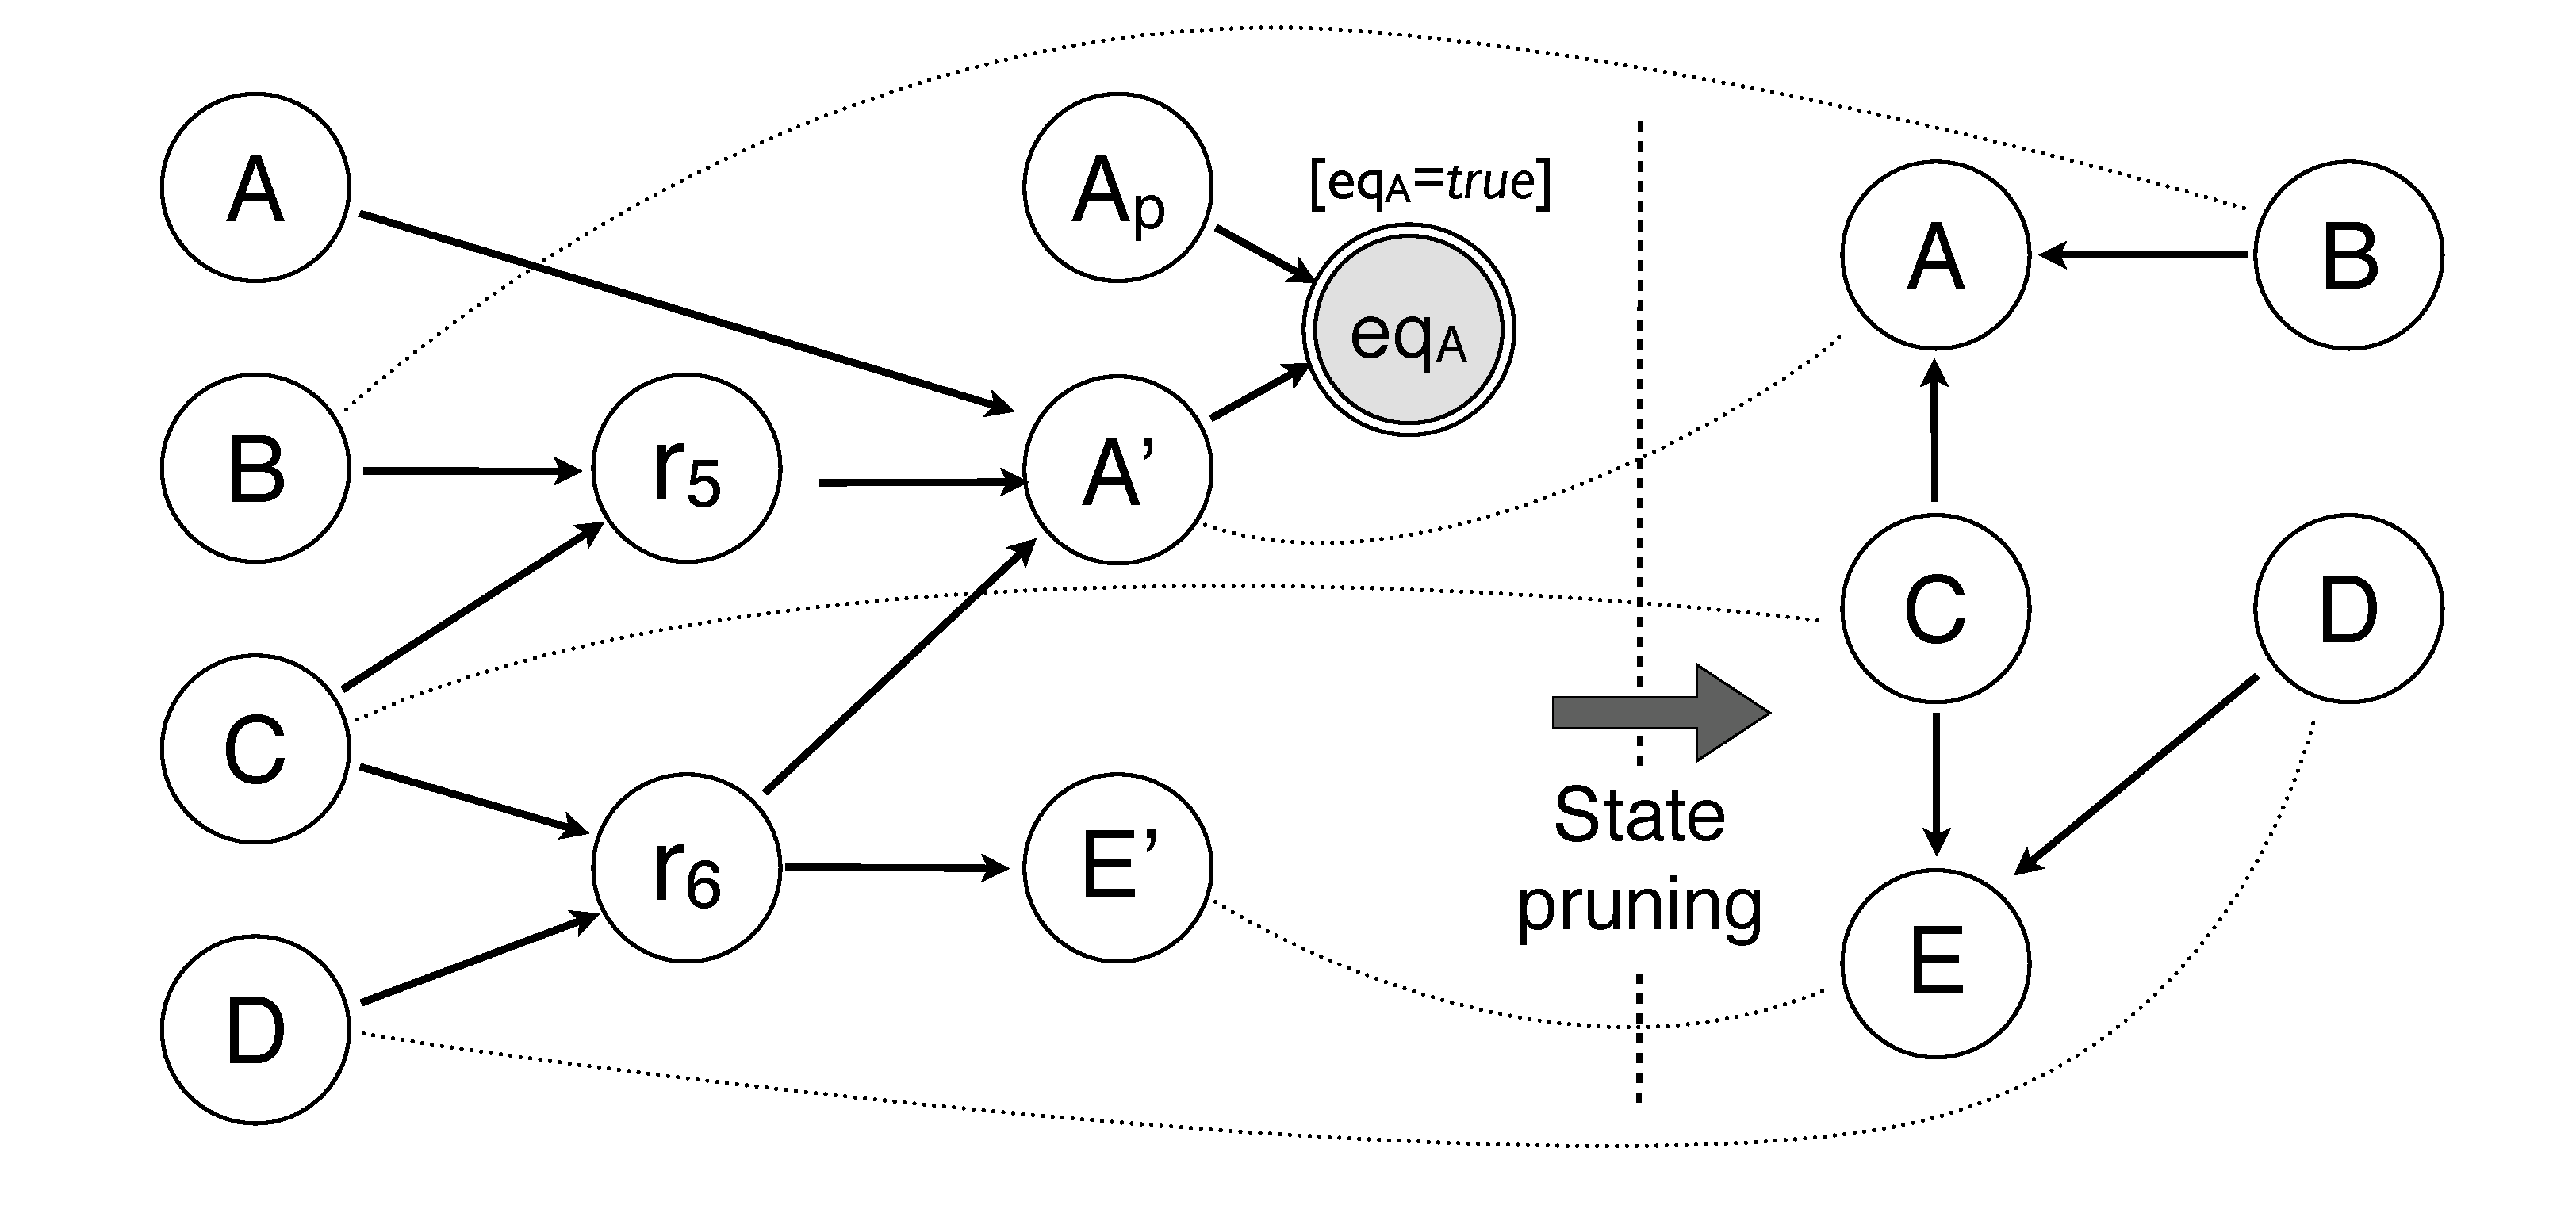
\includegraphics[scale=0.23]{imgs/pruning.pdf}
\caption{Illustration of the state pruning process. Only the nodes $A'$, $B$, $C$, $D$, $E'$ are retained. The dotted lines denote the correspondence between nodes.}
\label{fig:pruning}
\end{figure}


\subsection{Detailed example}
\label{sec:detailedexample}

To make the update procedure more concrete, we describe below a minimal but complete example of a workflow for a short interaction, detailing step-by-step how the dialogue state is updated in practice and employed to select the system actions. 

\subsubsection*{Description}

Assume a domain similar to the one shown in Figure \ref{fig:fsa}, where a user can request a robot to move forward, backward, left, right, or stop.  The set of dialogue acts $a_u$ that can be recognised by the system in this minimal example is the following: 
\begin{center}
$\{\mathit{Request(Forward)}$, $\mathit{Request(Backward)}$, $\mathit{Request(Left)}$, \\ $\mathit{Request(Right)}$, $\mathit{Request(Stop)}$, $\mathit{Other}\}$. \\
\end{center}
The corresponding system actions $a_m$ are: 
\begin{center}
$\{\mathit{Move(Forward)}$, $\mathit{Move(Backward)}$, $\mathit{Move(Left)}$, \\ $\mathit{Move(Right)}$, $\mathit{Move(Stop)}$, $\mathit{AskRepeat}\}$. 
\end{center}
The objective of the system is to fulfil the user command if it is reasonably confident regarding which action to execute.  Otherwise, the system asks the user to repeat. 

\subsubsection*{Domain specification}

The domain specification for this constructed example comprises an empty initial state and two rule-structured models $m_1$ and $m_2$: \begin{itemize}
% = \langle \langle a_u \rangle, \langle r_9, r_{10} \rangle \rangle$
\item Model $m_1$ is triggered by $a_u$ and includes two utility rules $r_{9}$ and $r_{10}$:
\begin{align*}
r_{9}: \ \ & \forall y, \\ 
& \textbf{if} \ (a_u = Request(y)) \ \textbf{then} \\ 
& \; \; \begin{cases} 
U(a_m' = Move(y)) = 2 \\ 
\end{cases} \\
& \textbf{else} \\ 
& \; \; \begin{cases} 
U(a_m' = Move(y)) = -2 \\ 
\end{cases} \\[4mm]
r_{10}: \ \ &  \; \; \begin{cases} U(a_m' = \mathit{AskRepeat}) = 0.5 \end{cases}
\end{align*}

Rule $r_{9}$ specifies that the utility of executing the action corresponding to the user command is 2, with a penalty of $-2$ when the wrong action is executed. Rule $r_{10}$ assigns a utility of 0.5 for asking a clarification question.\footnote{As the action selection process presented thus far does not perform forward planning, the utilities provided in this example correspond to long-term expected utilities (Q-values in the reinforcement learning terminology).}

%= \langle \langle a_m \rangle, \langle r_{11} \rangle \rangle
\item Model $m_2$ is triggered by $a_m$ and has one single predictive rule $r_{11}$: 
\begin{align*}
r_{11}: \ \ & \forall y, \\ 
& \textbf{if} \ (a_m = \mathit{AskRepeat} \land a_u=y) \ \textbf{then} \\ 
& \; \;  \begin{cases} 
P(a_{u}^{p\prime} = y) = 0.9 \\ 
\end{cases}
\end{align*}
Rule $r_{11}$ specifies that the probability that the user will repeat the last utterance when asked by the system to do so is expected to be $0.9$. Note the superscript $p$ in the random variable $a_{u}^{p\prime}$, which indicates that the effect expresses a prediction on a future dialogue act $a_u$.  
\end{itemize}

\subsubsection*{Processing workflow}

We now detail the processing workflow associated with a short (artificial) interaction:

\begin{dialogue} 
\speak{User } Now move forward \\ $\phantom{b}$ \textit{Hypotheses for} $\tilde{a}_u = [ (\mathit{Request(Forward)}, 0.6), (\mathit{Request(Backward)}), 0.4)]$  \\[-3mm]
\speak{System } Could you please repeat? \\[-3mm]
\speak{User } Please move forward! \\ $\phantom{b}$ \textit{Hypotheses for} $\tilde{a}_u = [ (\mathit{Request(Forward)}, 0.7), (\mathit{Other}, 0.3) ]$ \\[-3mm]
\speak{System } OK, moving forward!
\end{dialogue}

The recognition hypotheses $\tilde{a}_u$ produced by the ASR/NLU components are indicated underneath each user utterance:

Figure \ref{fig:detailedexample} details the steps involved in the state update procedure that follows from the reception of dialogue act hypotheses from the natural language understanding component. 

%Note that the probability and utility distributions shown in the figure are marginalised on their dependent variables.

\begin{figure}[p]
\centering
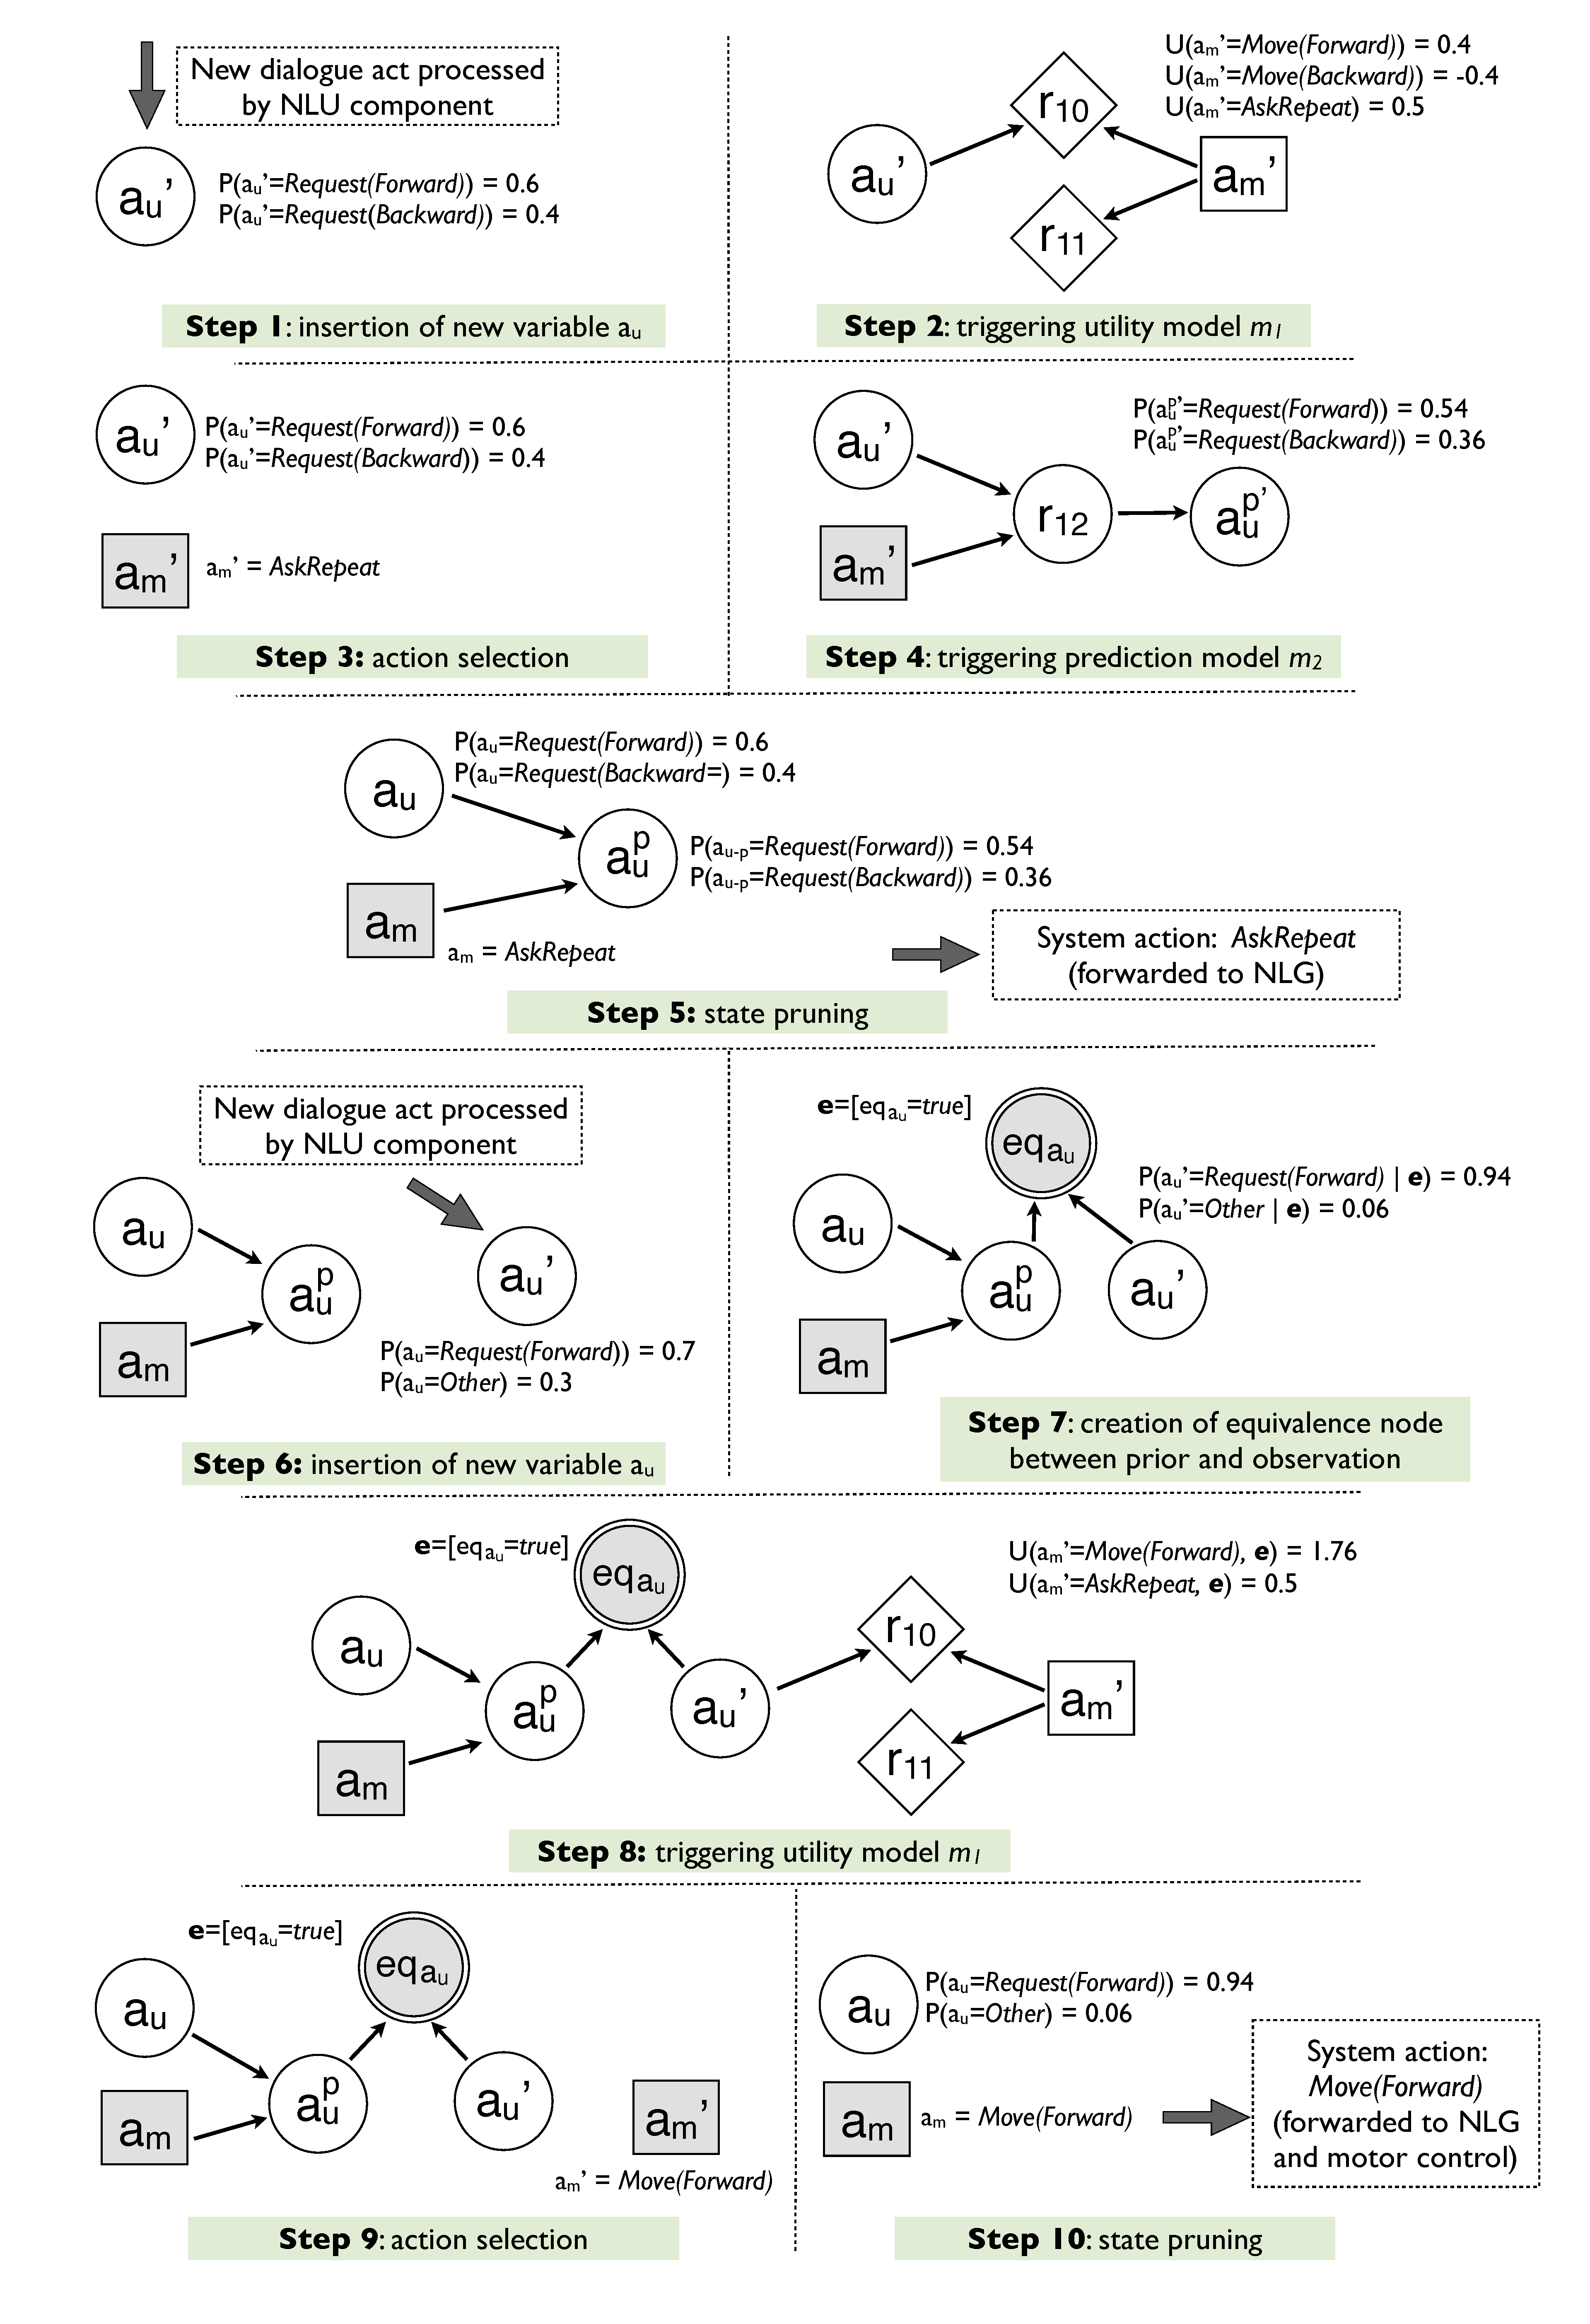
\includegraphics[scale=0.238]{imgs/detailedexample.pdf}
\caption{Detailed example of processing workflow. }
\label{fig:detailedexample}
\end{figure}
 
Step 1 inserts the new dialogue act hypotheses in the dialogue state.  This insertion triggers 
the utility model $m_1$. The instantiation results in Step 2 in the creation of two utility nodes and one decision node.  The optimal action to perform in this case is $\mathit{AskRepeat}$, which is selected by the system in Step 3. The action selection triggers model $m_2$ in Step 4, which creates a prediction node $a_{u}^{p\prime}$ expressing the expected probability distribution for the next user dialogue act. The state is finally pruned of the intermediary rule node in Step 5.  System components such as NLG can react on the updated state and generate the proper linguistic realisation of the system action. The system then waits for the user input, which is shown in Step 6.  The relation between the predicted and actual user response leads in Step 7 to the creation of an equivalence node, and the inclusion of the assignment $\mathit{eq}_{a_u} = true$ in the evidence. We notice that the combination of the prior distribution over predicted values and the actual distribution over dialogue act hypotheses increases the probability of $a_u' = \mathit{Request(Forward)}$. Step 8 triggers the model $m_1$ based on the new user input.  The best action at this processing stage is $\mathit{Move(Forward)}$, which is selected in Step 9.  This selection triggers model $m_2$, but rule $r_{11}$ is in this case irrelevant and is therefore directly deleted. Finally, the state is pruned of its intermediary nodes in Step 10, retaining only the last user and system actions $a_u$ and $a_m$. 

In comparison to the finite-state solution presented in Figure \ref{fig:fsa}, we observe that the rule-structured approach defined by models $m_1$ and $m_2$ allows the dialogue manager to accumulate evidence over time and prime the recognition hypotheses of the user dialogue act $a_u$ based on the previous dialogue act.  This accumulation of evidence is absent from the FSA, due to its rigid state representation and lack of extended memory. 

\section{Advanced modelling}
\label{sec:amodelling}

Dialogue domains often include random variables expressing specific data structures such as lists of elements or strings. The rule-based formalism described in the previous sections can be easily complemented with special-purpose tools to efficiently operate on these data structures. We first explain how conditions and effects can be defined on variables that represent lists, and then discuss how rules can manipulate strings. 

\subsection{Operations on lists}

Some state variables are best represented as lists of elements. For instance, the dialogue state may include random variables that enumerate  the $n$ most recent dialogue acts in the interaction history, the collection of tasks that must be executed, or the list of visual objects perceived by the system.  The range of values for such state variables is the power set of its possible elements. 

Special-purpose operators for the manipulation of such lists can be integrated in both the conditions and effects of probabilistic rules: 
\begin{itemize}
\item The syntax of rule conditions (see Table \ref{table:syntaxconditions}) can be extended to include operators to check the presence or absence of particular elements in a list, such as $a \in A$ or $a \notin A$. 
\item Rule effects can also be augmented to manipulate elements from a list.  Three new types of effects are created to this end, in addition to the traditional assignment of output values: \textit{add effects} (adding an element to a list), \textit{delete effects} (deleting an element from a list) and \textit{clear effects} (clearing all elements of a list). This is also realised by extending the syntax of rule effects (Table \ref{table:syntaxeffects}) to include these three types of effects. 
\end{itemize}

Figure \ref{fig:seteffects} illustrates two rules that apply these new effects to update a state variable $A$. 
 
\begin{figure}[ht]
\centering
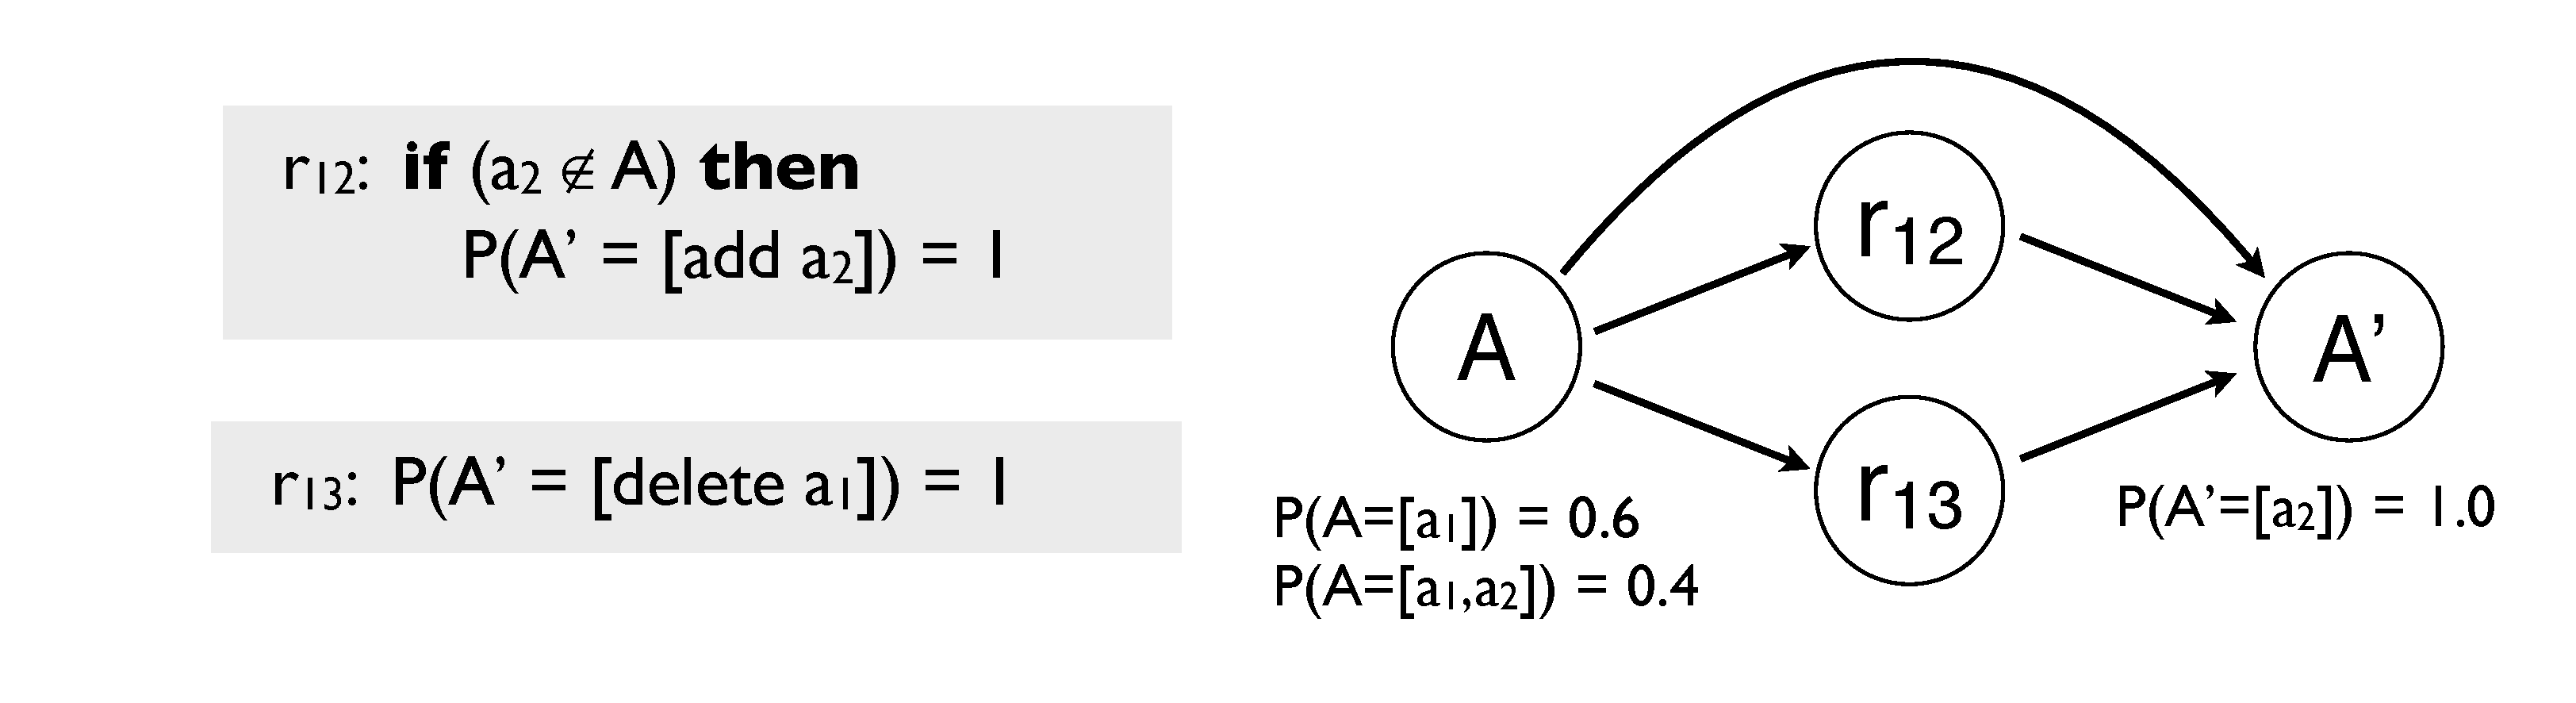
\includegraphics[scale=0.25]{imgs/seteffects.pdf}
\caption{Example of rules using add/delete effects to manipulate lists.}
\label{fig:seteffects}
\end{figure}

These new effects can be incorporated to the framework through a simple modification of the output distribution. Let $\mathbf{e}$ denote as before the conjunction of all effects $e_1 \land \dots \land e_n$. In addition to the previously defined set of values $\mathbf{e}(X)$ assigned for the variable $X$, we construct two new sets of values $\mathbf{e}_{add}(X)$ and $\mathbf{e}_{del}(X)$ that represent the values that are respectively added and deleted for the variable $X$ through the new effects we just described. The set $\mathbf{e}_{del}(X)$ includes all values for $X$ if the clear effect is applied. 

The output distribution in Equation \eqref{eq:outputdist2} is then rewritten as:
\begin{align}
&P(X'\!=\!x' \, | \, r_1\!=\!e_1, \dots, r_n\!=\!e_n, X\!=\!x) = \hspace{5cm} \nonumber \\ & \; \; \; \; \; \; \; \; \; \;  \begin{dcases} 
\frac{ \mathbf{1}(x' \in {\mathbf{e}(X')})} { |\mathbf{e}(X')| }  & \text{if } \mathbf{e}(X')\!\neq\!\emptyset \\
\mathbf{1}(x' = \left(\mathbf{e}_{add}(X') \cup \left(x \; / \; \mathbf{e}_{del}(X')\right)\right)) & \text{otherwise} \\
\end{dcases}\label{eq:outputdist4}
\end{align} 

The output distribution associated for a new variable (cf. Equation \eqref{eq:outputdist1}) can be rewritten in a similar manner.

%The assignment effects in $\mathbf{e}(X)$ and the add/delete effects in $\mathbf{e}_{add}(X)$ and $\mathbf{e}_{delete}(X)$ being mutually incompatible, the assignment effects are assumed to take precedence.

%Lists are defined to be equal if they include the same elements in the same order.

%Other types of collections such as sets with no duplicate elements can be exploited in the same manner. 

\subsection{Operations on strings}

Many of the data structures present in the dialogue state are strings -- the most prominent ones being the last user utterance $u_u$ and the last system utterance $u_m$. The integration of special-purpose functions for manipulating strings within the conditions and effects of probabilistic rules is therefore desirable. In particular, rules can be extended to perform template-based string matching operations.  The idea is to include a new type of conditions that checks whether a string matches a given template. Templates can include slots to fill, which are conceptually similar to the quantified variables discussed in Sections \ref{sec:quantification}. A successful match will thus generate values for the filled slots, which will be included as part of the groundings for the rule.  Both full and partial matching can be employed.

Figure \ref{fig:stringmanip} illustrates how such templates are applied in practice.  $\{\mathit{OBJ}\}$ denotes a slot that is to be filled through matching the template with the value specified in $u_u$. 
\begin{figure}[ht]
\centering
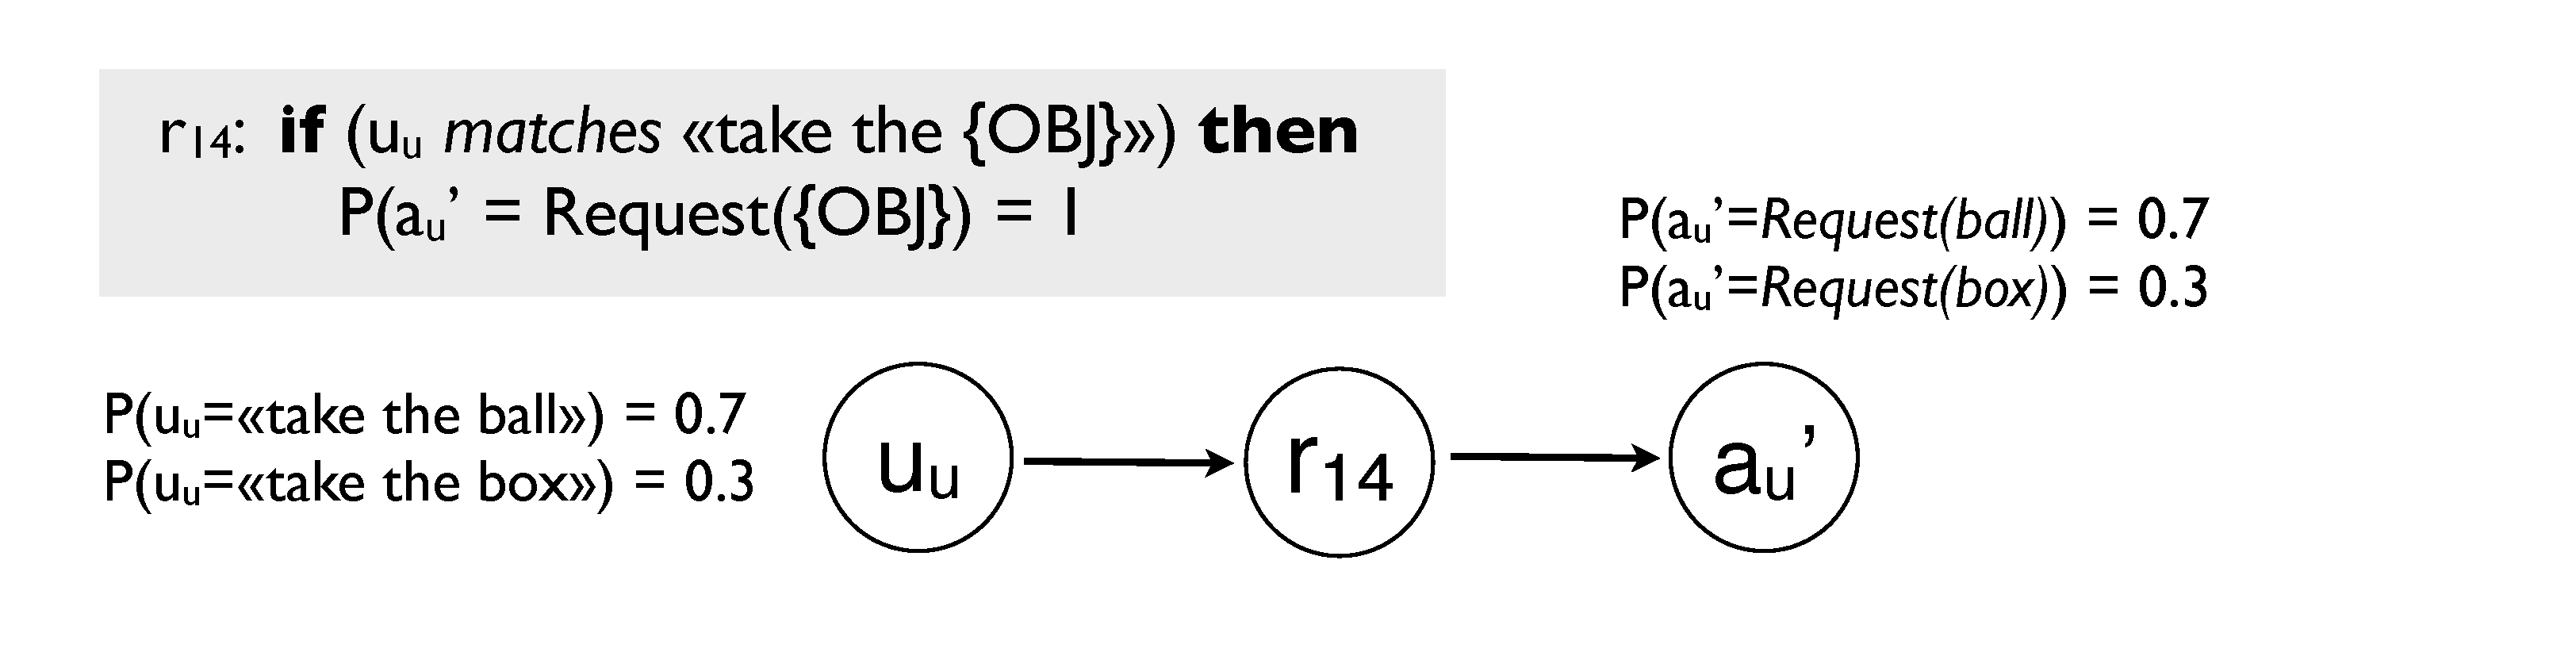
\includegraphics[scale=0.25]{imgs/stringmanip.pdf}
\caption{Example of rule using string matching operations.}
\label{fig:stringmanip}
\end{figure}

\section{Relation to previous work}
\label{sec:relatedwork}

The idea of using structural knowledge in probabilistic models has been explored in many directions, both in the fields of decision-theoretic planning and reinforcement learning \citep{Hauskrecht98,Pineau:2004,KerstingR04,lang10jair,Otterlo2012}, and in statistical relational learning\index{statistical relational learning}\index{decision-theoretic planning} \citep{Jaeger01,Richardson:2006,getoor:srlbook07}.  The introduced structure may be hierarchical, relational, or both. As in our approach, most of these frameworks rely on the use of expressive representations serving as templates for the generation of classical probabilistic models.  The surveys of \cite{Otterlo2006,Otterlo2012} provide a complete overview of relational and first-order logical approaches for reinforcement learning in Markov decision processes, covering both model-free and model-based methods.  While the formalisation presented in this thesis and the aforementioned approaches share many insights, they also reveal several interesting differences: 

\begin{itemize}

\item Probabilistic rules are primarily tailored for dialogue management tasks and seek to capture dialogue domains by striking a balance between propositional and first-order logic.\index{first-order logic} The formalism deliberately eschews the complexity of full-scale first-order probabilistic inference to ensure that the domains models can be applied under real-time constraints. This design choice sets it apart from other frameworks such as Markov logic networks\index{Markov logic network} which can express arbitrary first-order formulae but are often tedious to instantiate due to the size and complexity of the resulting models.\footnote{Although see \cite{Kennington:2012} for an approach that applies Markov logic networks to incremental natural language understanding for dialogue.} 

\item Probabilistic rules are also designed to operate under partially observable settings\index{partial observability}, as state uncertainty is a pervasive and unavoidable aspect of verbal interactions.  By contrast, most previous work on relational probabilistic models are limited to fully observable environments, with the exception of some limited theoretical studies by \cite{Wang:2010} and \cite{SannerK10}. 

\item Finally, the presented framework posits that the \textit{if...then...else} skeletons of probabilistic rules are best encoded by the system designers based on their expert knowledge of the domain, while the rule parameters can be estimated empirically. We therefore exclude the problem of structure learning from the scope of this thesis, as opposed to several approaches in which the domain rules and constraints are extracted via machine learning techniques \citep{PasulaZK07,Kok:2009}.

\end{itemize}

Probabilistic rules also bear similarities with planning description languages such as the Planning Domain Definition Language\index{Planning Domain Definition Language} \citep[PDDL, see ][]{mcdermott1998} and its probabilistic extension, the Probabilistic Planning Domain Definition Language \citep[PPDDL, see ][]{younes2004ppddl1}.  These languages are structured through action schemas that specify how (parametrised) actions can yield particular effects under various conditions. As in probabilistic rules, these languages try to carefully balance between the language expressivity and the complexity of the planning algorithm, based on a limited form of first-order logic. A relational extension of PDDL, named RDDL, has also been introduced in recent planning competitions \citep{Sanner:RDDL}. The learning techniques presented by \cite{PasulaZK07} to estimate transition functions based on noisy indeterministic deictic rules are directly related to our approach, as is the recent work of \cite{lang10jair} on probabilistic noisy planning rules.   Both frameworks define conditions associated with probabilistic distributions over effects. Their approaches are, however, restricted to fully observable settings. 

In the dialogue management literature, most structural approaches rely on a clear-cut task decomposition into goals and sub-goals \citep{Allen:2000:AGD:973935.973937,Steedman-Petrick:07,Bohus:2009}, where the completion of each goal is assumed to be fully observable, discarding any remaining uncertainty.  Our own work on multi-policy dialogue management in \cite{multipolicy-sigdial2011} relaxes the assumption of perfect knowledge of task completion, handling multiple policies as a problem of probabilistic inference over activation variables.  Probabilistic rules can be considered an extension of this early work, where the structural knowledge is not confined to task decomposition but is extended to generic rules over state variables.  

The processing workflow presented in this chapter is strongly inspired by information state\index{information state} approaches to dialogue management \citep{Larsson:2000,Bos2003}, which are also based on a shared state representation that is updated according to a rich repository of rules.  \cite{Ginzburg2012} also models conversational phenomena by way of update operations that are encoded with rules mapping conditions to effects. However, contrary to the framework presented here, the rules specified in these approaches are generally deterministic and do not include learnable parameters. The action selection mechanism is also conceptualised slightly differently, as information-state frameworks rely on rules that directly select the most appropriate action given the current state. By contrast, probabilistic rules adopt a decision-theoretic approach that decomposes action selection in two stages: utility rules first determine the utility distributions associated with the space of possible system actions in the current dialogue state, after which the system searches for the action that yields the maximum expected utility on the basis of these distributions.  

The literature on dialogue policy optimisation with reinforcement learning also contains several approaches dedicated to dimensionality reduction\index{dimensionality reduction} for large state--action spaces, such as function approximation \citep{Henderson:2008}, hierarchical reinforcement learning \citep{Cuayahuitl:2010} and summary POMDPs \citep{Young:2010}.  Many of these techniques have already been discussed in Section \ref{sec:application-dm} and will therefore not be repeated here. Most current approaches in dialogue policy optimisation focus on large but weakly structured state spaces (generally encoded as large lists of features), which are suited for slot-filling dialogue applications but are difficult to transfer to more open-ended or relational domains.  The idea of state space partitioning\index{state space!partitioning of}, implemented here via high-level conditions, has also been explored in recent papers \citep[see e.g.\ ][]{Williams2010}. \cite{Crook:2010} explored the introduction of complex user goal states including disjunction and negation operators. \cite{Heriberto2011} describes a policy optimisation approach based on logic-based representations of the state--action space for relational MDPs. The main difference to our approach lies in his reduction of the belief state to fully observable variables whereas we retain the partial observability associated with each variable.  The work of \cite{Mehta:2010} and \cite{Raux2011} demonstrated how tree-structured Bayesian networks called probabilistic ontology trees can improve belief tracking performance.  The tree structure is derived in their work from a hierarchical concept structure.  Finally, \cite{neill2011} describe a procedure for the selection of dialogue strategies based on probabilistic logic programming. 

\section{Conclusion}

This chapter has presented the formalism of probabilistic rules, which forms the core of the modelling approach developed in this thesis. We started by arguing that dialogue models are often highly structured, and that this structure can be leveraged by introducing latent variables, partitioning value assignments for the parent variables, and making use of quantification. We then explained how these structural insights can be transferred into a new computational framework -- to which we gave the name of probabilistic rules -- that combines concepts borrowed from both first-order logic\index{first-order logic} and probability theory in order to get ``the best of both worlds'', i.e.\ a representation formalism that is both richly expressive and capable of capturing uncertain knowledge.  These rules are practically defined as \textit{if...then...else} constructions that associate high-level conditions on input variables to probabilistic effects on output variables.  Multiple extensions of the formalism have been developed to e.g.\ encode utility distributions, enclose universal quantifiers, and efficiently manipulate data structures such as lists of elements and strings.

At runtime, these rules are instantiated in the Bayesian network representing the current dialogue state. The instantiation procedure creates a latent node for each rule, which is conditionally dependent on the input variables of the rule.  For probability rules, this node is a chance node that expresses a probability distribution over the possible effects of the rule. Utility rules are similarly instantiated with a utility node expressing the utility distribution for specific decision variables.  Universally quantified variables can be included in the conditions and effects of the rules, allowing particular aspects of the rule to be underspecified. The rules are grouped into models that are attached to the dialogue state and are triggered upon relevant state updates. 

Probability and utility rules effectively function as high-level templates for the definition of a dynamic decision network (such as the ones used in MDPs and POMDPs). The expressive power of these rules allows them to efficiently encode complex relations between variables, and thereby reduce the number of parameters to estimate.  We have, however, not yet detailed how this parameter estimation is practically performed. The next two chapters provide answers to this important question. 
